\onehalfspacing

\section{Lösungsansatz}

Bei der prototypischen Lösung steht im Zentrum dieser Arbeit die Wissensdatenbank \textit{Wikidata}\footnote{URL: \url{https://www.wikidata.org/wiki/Wikidata:Main_Page} (letzter Zugriff am 20.05.2022).} als offener Forschungsdatenmanagement-Service. Bei Wikidata handelt sich ursprünglich um ein offenes dankenbankbasiertes Angebot von Wikimedia für strukturierte Daten im Wiki*versum, das das Konzept von Linked Open Data umsetzt. Damit ist es flexibel und sprachenunabhängig einsetzbar, wodurch es als Modell auch für Forschungsdatenmanagement in der akademischen Wissenschaft interessant wird. Tatsächlich wird dieser Weg im Rahmen von NFDI gegenwärtig bestritten. Das \textit{Open Science Lab} am ,,Leibniz-Informationszentrum Technik und Naturwissenschaften und Universitätsbibliothek''\footnote{URL: \url{https://www.tib.eu/de/} (letzer Zugriff am 20.05.2022).} hat für das Konsortium \textit{NFDI4Culture}\footnote{URL: \url{https://nfdi4culture.de/index.html} (letzter Zugriff am 20.05.2022).} Wikidata und insbesondere die zugrunde liegende Software \textit{Wikibase}\footnote{URL: \url{https://wikibase.consulting/what-is-wikibase/} (letzter Zugriff am 20.05.2022).} auf die Einsetzbarkeit für ein Forschungsdatenmanagement von Kulturdaten hin evaluiert. Erste Ergebnisse wurden im März 2022 auf dem TIB-Blog veröffentlicht.\footnote{Siehe Lozana Rossenova (2022): Examining Wikidata and Wikibase in the context of research data management applications, veröffentlicht am 16.03.2022 auf dem TIB-Blog, URL: \url{https://blogs.tib.eu/wp/tib/2022/03/16/examining-wikidata-and-wikibase-in-the-context-of-research-data-management-applications/}.} Parallel führt das NFDI4Culture-Konsortium selbst die Workshop-Reihe ,,Wikibase'' durch.\footnote{URI: \url{https://nfdi4culture.de/resource/E2261/about.html}.} 

Auch im Kontext historischer Forschung kommt Wikidata bereits zum Einsatz. Das Online-Portal ,,Archivführer. Deutsche Kolonialgeschichte'' nutzt Wikidata als strukturierte Datenbasis für in Zusammenhang mit dem Thema ,,Deutsche Kolonien und Schutzgebiete'' stehende Forschungsdaten.\footnote{Das Projekt wurde 2017 an der Fachhochschule Potsdam initiiert und ist vom Auswärtigen Amt gefördert worden, URL: \url{https://archivfuehrer-kolonialzeit.de/} (letzter Zugriff am 20.05.2022).} Das Portal führt lediglich die Wikidata-Daten für die Datenpräsentation zusammen und ermöglicht einen multiperpektivischen Zugang zu den Daten.\footnote{Zum Beispiel Georeferenzierung der Orte anhand historischen Kartenmaterials, URL: \url{https://archivfuehrer-kolonialzeit.de/map} (letzter Zugriff am 20.05.2022).} Die Besonderheit ist, dass die Datenbereitstellung durch Wikidata ermöglicht, über die Projektlaufzeit hinaus Daten von jeder/jedem erweitern zu lassen sowie diese in gänzlich anderen Kontexten zu verwenden. Darüber hinaus verfolgt das Projekt das Ziel, die Daten mit der ,,kolonialen Vergangenheiten anderer Ländern''\footnote{URL: \url{https://archivfuehrer-kolonialzeit.de/about} (letzter Zugriff am 20.05.2022).} zu verknüpfen und auf diese Weise das Forschungsfeld zum Deutschen Kolonialismus anschlussfähig an die Forschung zum Europäischen Kolonialismus zu machen. Die Zusammenarbeit und der kollaborative Austausch dazu erfolgen ebenfalls global in Wikidata mit dem ,,Wikidata:WikiProject European Colonialism''.\footnote{URL: \url{Wikidata:WikiProject European Colonialism} (letzter Zugriff am 20.05.2022).} Das internationale Projekt ,,European Holocaust Research Infrastructure'' (EHRI), welches im Rahmen der Open Science-Strategie von der Europäischen Kommission seit 2017 gefördert wird\footnote{Im EU-Programm ,,Horizon Europe'', das bis 2027 läuft, URL: \url{https://ec.europa.eu/info/research-and-innovation/funding/funding-opportunities/funding-programmes-and-open-calls/horizon-europe_en}. Projektwebsite von EHRI, URL: \url{https://www.ehri-project.eu/} (alle letzter Zugriff am 20.05.2022).} nutzt Wikidata als zentrales Verzeichnis zur Erstellung einer Liste von Ghettos aus der Zeit des Holocausts.\footnote{Nancy Cooey (2018): Using Wikidata to build an authority list of Holocaust-era ghettos, veröffentlicht am 12.02.2018 auf dem EHRI Document Blog, URL: \url{https://blog.ehri-project.eu/2018/02/12/using-wikidata/\#Selecting\_Wikidata\_as\_a\_Tool} (letzter Zugriff am 20.05.2022).} Ziel ist, Daten aus verschiedenen Enzyklopädien, die bisher isoliert waren, in Wikidata erstmals zusammenzuführen und zu verknüpfen.\footnote{Vgl. ebd. Zentrale Enzyklopädien sind ,,The Yad Vashem Encyclopedia of the Ghettos During the Holocaust'' von Yad Vashem (Israel) und ,,USHMM Encyclopedia of Camps and Ghettos'' des United States Holocaust Memorial Museum (USA).}

Grundsätzlich ist bei der Implementierung des offenen Forschungsdatenmanagements mit Wikidata ist zu beachten, dass hier das Konzept von Linked (Open) Data umgesetzt wird, bei dem es sich, wie in Kapitel 2.2.2 bereits erläutert wurde, um einen wesentlichen Baustein des \textit{Semantic Web} handelt. Damit erfolgt offenes FDM in der höchsten Open Data-Stufe (= 5 Sterne). Vorteil ist, dass die Stärken dieses Konzepts, welche vor allem in der Verknüpfung und Vernetzung von Daten liegen, für das Forschungsdatenmanagement ausgenutzt werden können. Nachteilig ist, dass dieser Ansatz voraussetzungsreicher als andere Lösungen ist, da zum einen Kenntnisse der allgemeinen Technologien von Linked Data Web wie RDF (Resource Description Framework), JSON-LD (JavaScript Object Notation for Linked Data) oder URI (Uniform Ressource Identifier)\footnote{Im Rahmen dieser Arbeit können diese Technologien nicht detailliert vorgestellt werden, daher wird zur Vertiefung auf die Grundlagenliteratur verwiesen. Siehe zum Beispiel Malte Rehbein: Ontologien, in: Fotis Jannidis, Hubertus Kohle, Malte Rehbein (Hrsg.), Digital Humanities, 2017, doi:10.1007/978-3-476-05446-3\_11; Christian Stein: Linked Open Data – Wie das Web zur Semantik kam, in: Bibliothek Forschung und Praxis (Hrsg.), Band 38, Nr. 3, 2014, S. 447-455, doi:10.1515/bfp-2014-0055; Patrick Danowski, Adrian Pohl: (Open) Linked Data in Bibliotheken, Berlin, Boston, 2013, doi:10.1515/9783110278736; Gradmann, Steffen Hennicke, Marlies Olensky: Linked Data, in: Digitale Dienste für die Wissenschaft (Hrsg.), 2012, S. 18-22, doi.org/10.18452/6627;  } und zum anderen Kenntnisse des spezifische Metadatenschemas bzw. der Onotologie zugrunde liegenden Software Wikibase von Wikidata.\footnote{Siehe Mediawiki (2022): Wikibase/DataModel, URL:\url{https://www.mediawiki.org/wiki/Wikibase/DataModel} (letzter Zugriff am 22.05.2022).} für die Umsetzung benötigt werden. Kurzgefasst ist im Wesentlichen zu beachten, dass jegliche Modellierung von Daten graphenbasiert in sogenannten Tripeln als Subjekt-Prädikat-Ausdrücke erfolgt, was sich grundlegend von der konventionellen tabellenbasierten relationalen Datenmodellierung mit Tupeln unterscheidet. In Wikidata werden diese Ausdrücke als Aussagen (Statements) bezeichnet. Mit ihnen können Konzepte inhaltlich erschlossen werden.\footnote{Siehe Wikidata Statements, URL: \url{https://www.wikidata.org/wiki/Help:Statements} (letzter Zugriff am 27.05.2022).}

\section{Erhebung}

\begin{quote}
    [...] Dass dieses methodisches Vorgehen auch transparent und nachvollziehbar ist.\footnote{B4\_Transkript, Pos. 67.}

    [...] Das große Problem ist, was ist in Gottes Namen ein jüdisches Unternehmen.\footnote{B1\_Transkript, Pos. 147.}
\end{quote}

Datenerhebung in der empirischen historischen Forschung geht mit historischer Quellenanalyse und Quellenkritik einher.\footnote{Vgl. W. H. Schröder: Historische Sozialforschung: Forschungsstrategie - Infrastruktur - Auswahlbibliographie.
Historical Social Research, in: Supplement (Hrsg.) 1988, Nr. 1, S. 1-109, hier S. 15ff., URN: \url{https://nbn-resolving.org/urn:nbn:de:0168-ssoar-286038}
} Anders als in der naturwissenschaftlichen Datenerhebung, wo anhand von Experimenten, Beobachtungen, Simulationen oder Messungen, Daten in Echtzeit gewonnen werden und dementsprechend die Erhebungsmethoden an den Forschungsfragen angepasst werden können, ist die Vorgehensweise bei den geschichtswissenschaftlichen Disziplinen maßgeblich von der Überlieferungstruktur und der Quellensituation abhängig.\footnote{Was zu einem ,,Quellenproblem'' führen kann, siehe dazu ebd. S. 19f.} Informationen zur Erhebung sind also essentiell, um Forschungsdaten im Sinne einer Datenkritik kontextualisieren, verstehen und damit letztlich bewerten zu können. Bei den Forschungsdaten zu jüdischen Gewerbebetrieben sind diese jedoch nicht hinterlegt und es handelt sich daher bisher um implizites Wissen, was eine Nachnutzung erschwert oder sogar unmöglich machen kann. Hinsichtlich der Nachvollziehbarkeit und Transparenz von Forschungsdaten ist daher Ziel von offenem Forschungsdatenmanagement, das Wissen um den Entstehungsrahmen sowie um die geschichtswissenschaftliche Datenerhebungsmethode explizit zu machen. Dabei soll das grundsätzliche methodische Definitionsproblem des Begriffs ,,jüdischer Gewerbebetrieb'' mitdiskutiert werden.

\subsection{Entstehungsrahmen}

Im Forschungsfeld ist der Großteil der Forschungsdaten zu jüdischen Gewerbebetrieben in lokalen wissenschaftlichen Forschungsprojekten erhoben worden, daher stellen vor allem sie die relevanten Informationen zum Entstehungsrahmen bereit. Die Frage, wie verschiedene (akademischen) Forschungsaktivitäten zur semantische Anreicherung von Forschungsdaten konzeptionalisiert und formalisiert werden können, scheint gegenwärtig noch nicht Gegenstand des Forschungsdatenmanagements zu sein, denn einen wissenschaftlichen Standard, nach denen diese beschrieben werden können und sollen, konnte nicht ermittelt werden. Zwar gibt es inzwischen generische Metadatenstandards wie \textit{Dublin Core} der \textit{Dublin Core Metadata Initiative}\footnote{URL: \url{https://www.dublincore.org/specifications/dublin-core/dcmi-terms/} (letzter Zugriff am 15.05.2022)} oder \textit{DataCite}\footnote{URL: \url{https://datacite.org/} (letzter Zugriff am 15.05.2022)} des gleichnamigen internationalen Konsortiums. ,,DublinCore'' fokussiert aber in erster Linie auf Informationen zur technischen Umsetzung sowie zur Veröffentlichung von digitalen Ressourcen und ist damit näher an der traditionellen Praxis der Formalerschließung in der Bibliothekskatalogisierung dran. ,,DataCite'' ist umfangreicher und lässt als optionale Elemente auch Angaben zu Fördermittelgebern zu.\footnote{,,Funding references'', siehe Data-Cite-Dokumentation auf GitHub URL: \url{https://github.com/UB-LMU/DataCite\_BestPracticeGuide/blob/master/BestPracticeGuide.md\#fundingreference} (letzter Zugriff am 23.05.2022).} Ein Konzept ,,Forschungsprojekt'' findet sich aber in beiden Standards nicht wieder. Dem gegenüber bietet Wikidata einen entscheidenden Vorteil: Zur Verbesserung strukturierter Beschreibungen von bestimmten Konzepten wie zum Beispiel ,,Mathematik'' oder ,,Astronomie'' können von der Wikidata-Community sogenannte \textit{Wikidata:Wikiprojekte} angelegt werden. Sie bieten die Möglichkeit der kollaborativen Modellierung und des gemeinsamen Austauschs. Dadurch kann ein festes Vokabular (Authority File) für ein Konzept in Wikidata angelegt werden, die allerdings nur informellen Charakter haben. Inzwischen gibt es eine Vielzahl an unterschiedlichen Projekten, die in Kategorien unterteilt sind.\footnote{Auch die NFDI sowie das Archivportal zum Deutschen Kolonialismus sind mit eigenen Projekten vertreten. Wikidata:WikiProject NFDI, URL: \url{https://www.wikidata.org/wiki/Wikidata:WikiProject_NFDI}.} In der Kategorie \textit{Category:Research WikiProjects} beschäftigt sich eine internationale Wissenschaftler*innengruppe mit der Abbildung des Konzepts ,,Forschung'' in Wikidata.\footnote{URL: \url{https://www.wikidata.org/wiki/Wikidata:WikiProject_Wikidata_for_research}. Darunter ist auch eine deutsche Gruppe, URL: \url{https://www.wikidata.org/wiki/Wikidata:WikiProject_Wikidata_for_research/de}.} Dort integriert ist das Unterprojekt \textit{Wikidata:WikiProject Wikidata for research/Data models/Research projects}, in dem sich ausschließlich mit dem Konzept ,,Forschungsprojekt'' befasst wird.\footnote{URL: \url{https://www.wikidata.org/wiki/Wikidata:WikiProject_Wikidata_for_research/Data_models/Research_projects}.} Hier zeigt sich die Stärke des gemeinschaftlichen Ansatzes von Wikidata besonders, denn die Chance, dass sich in Wikidata mit einem Problem schon befasst wird, ist sehr hoch.

\begin{figure}[h]
    \centering
    \frame{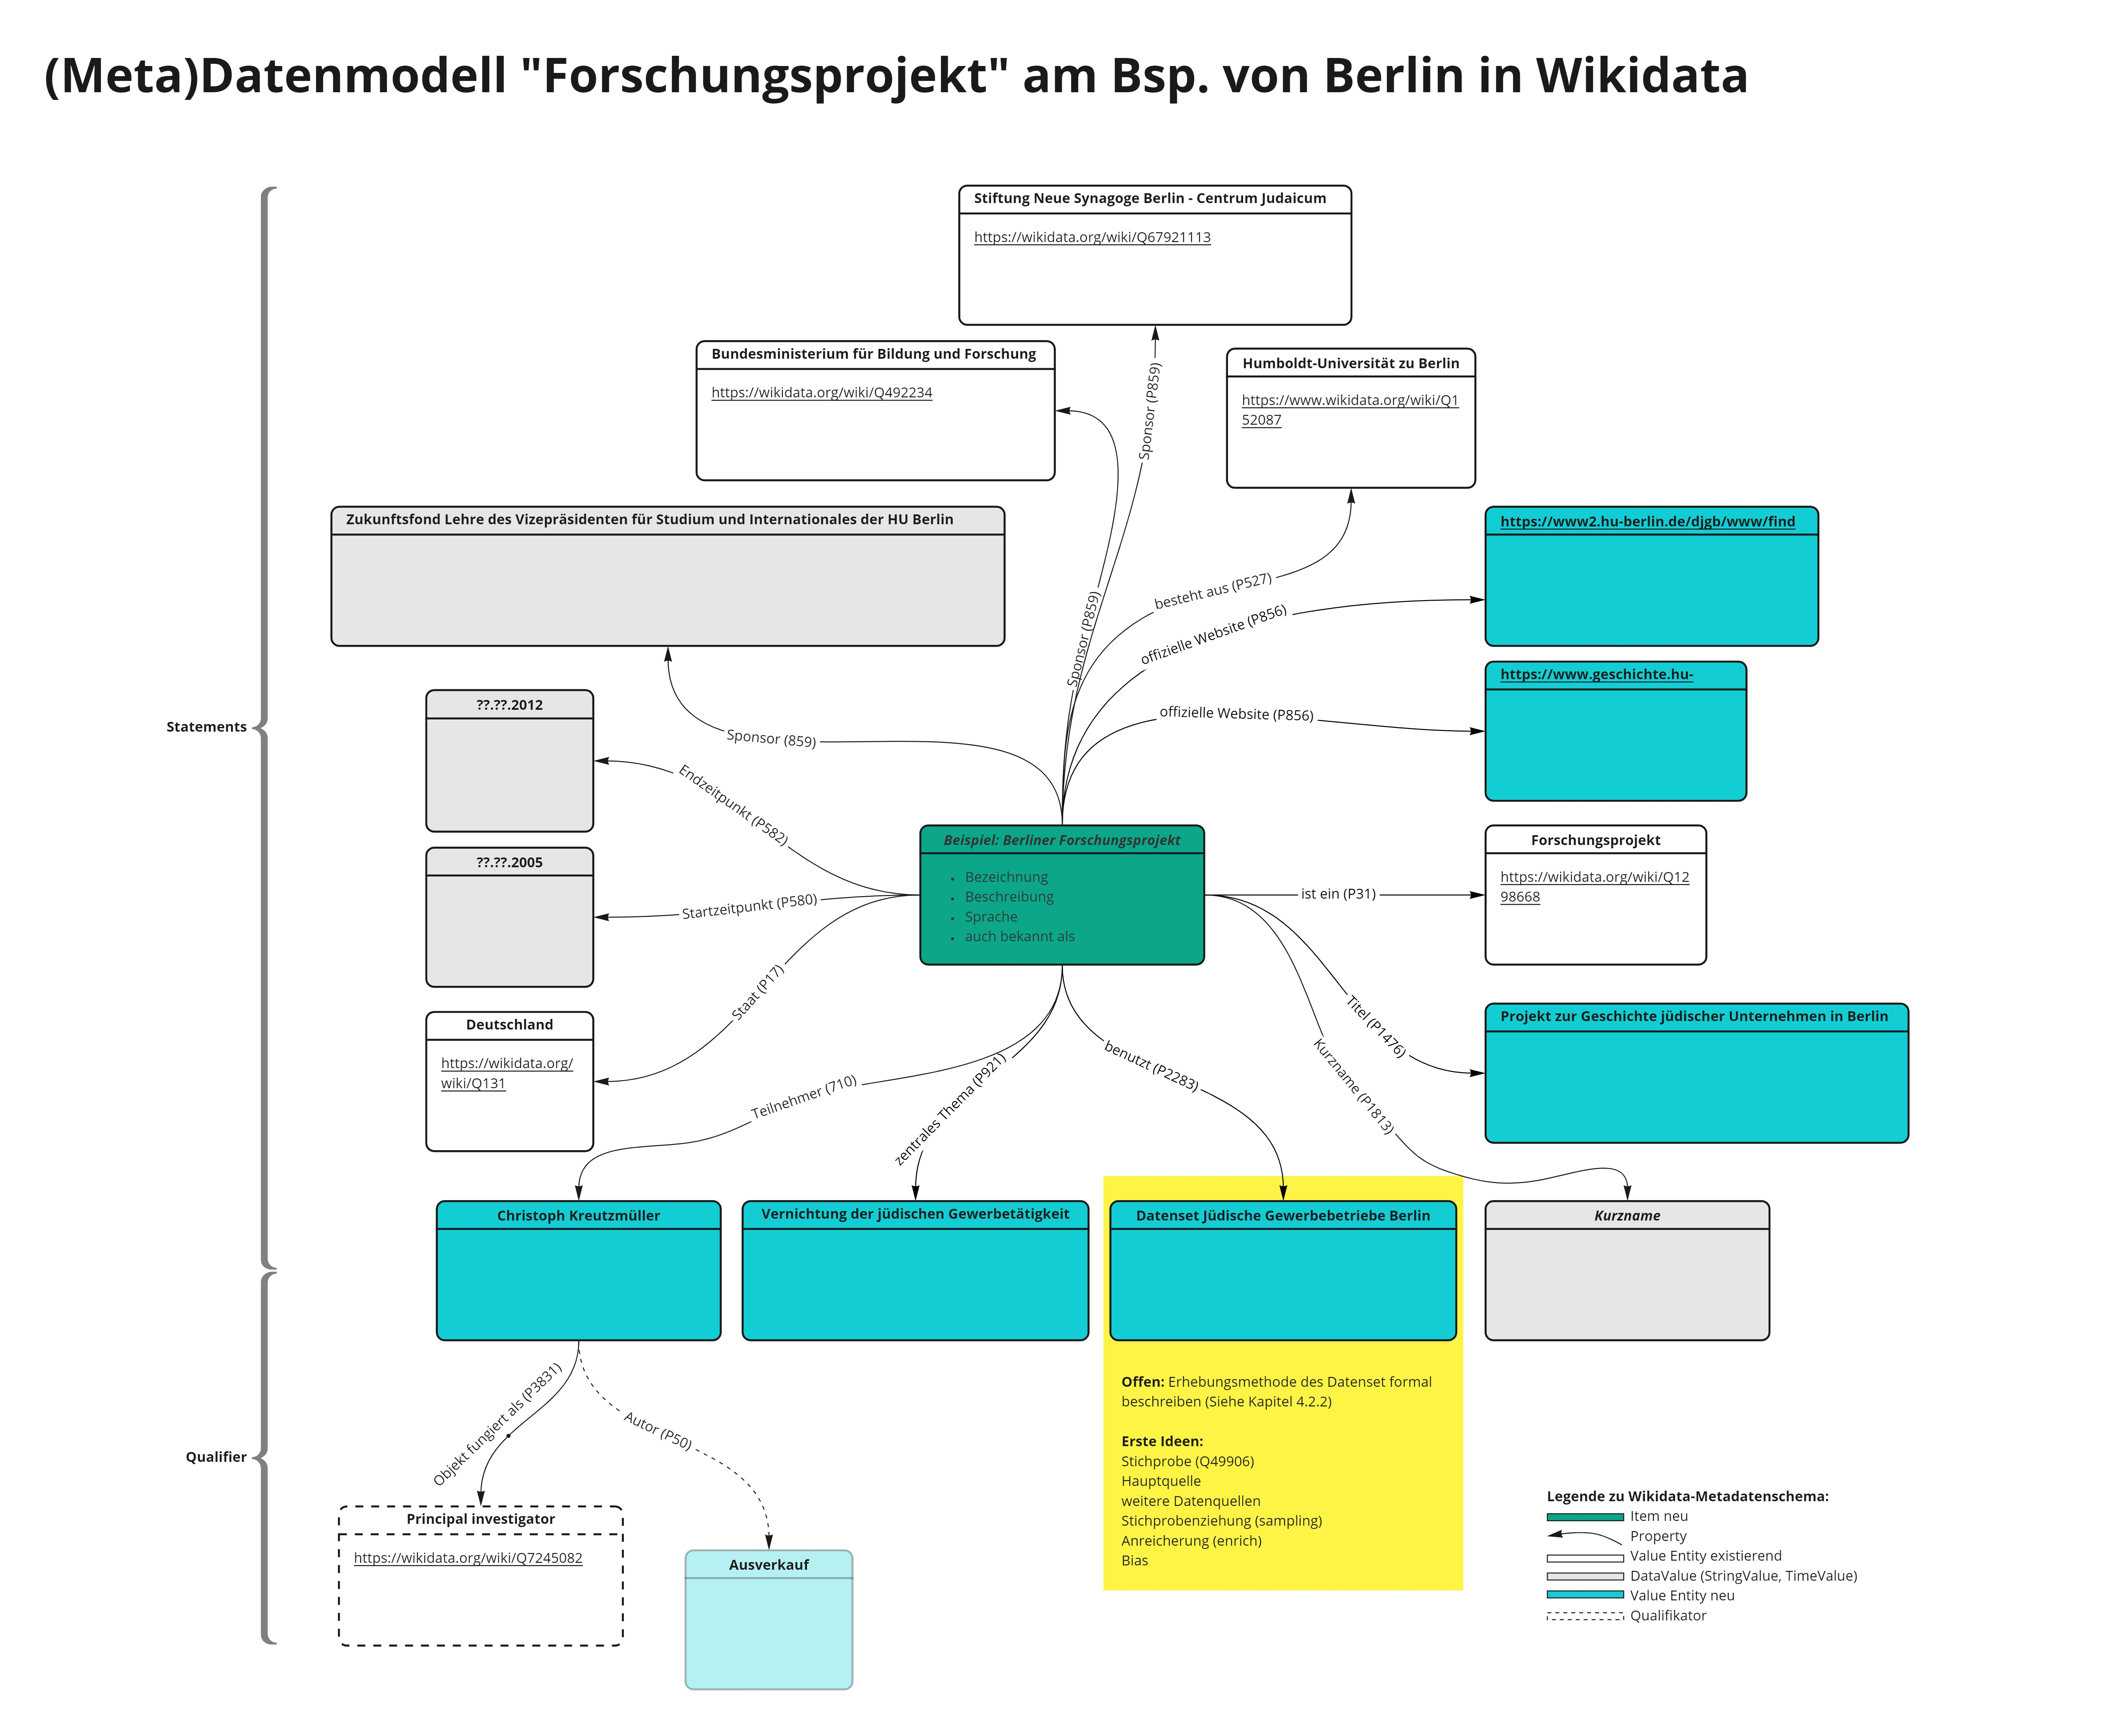
\includegraphics[width=\ScaleIfNeeded]{wikidata-item_research-project}}
    \caption{Modellierung der Forschungsprojekte in Wikidata.}
    \label{fig:x cubed graph} \footnotetext{Größere Darstellungen der Modellabbildungen sind alle separat nochmals im Anhang beigefügt.}
\end{figure}

Folglich wäre die eigene Modellierung von ,,Forschungsprojekt'' für die lokalen Forschungsprojekte im Forschungsfeld redundant, da diese von dem bestehenden Wikidata-Projekt abgeleitet werden kann (Abbildung 4.1).\footnote{Als Orientierung diente das Forschungsprojekt ,,Amyloid fibril cytotoxicity: new insights from novel approaches'', URL: \url{https://www.wikidata.org/w/index.php?title=Q52268104&oldid=1528020632}.} Aus dem Modell in Abbildung 4.1 geht darüber hinaus hervor, dass viele Entitäten in Wikidata bereits existieren und nicht neu angelegt werden müssen.\footnote{Entitäten mit weißem Hintergrund.} Auch die Verknüpfung von externen Information ist möglich. Die Deutsche Forschungsgemeinschaft (DFG) hat mit dem Informationssystem ,,GEPRIS – Geförderte Projekte der DFG'' (GEPRIS)\footnote{URL: \url{https://gepris.dfg.de/gepris/OCTOPUS?task=showAbout} (letzter Zugriff am 21.05.2022).} in Auszügen ihre Daten zu allen gegenwärtigen und vergangenen geförderten Projekten veröffentlicht. Dort ist auch das Forschungsprojekt ,,Geschichte mittlerer und kleiner jüdischer Unternehmen in Frankfurt am Main und Breslau 1929/39 bis 1945'' archiviert.\footnote{URL: \url{https://gepris.dfg.de/gepris/projekt/48308995?context=projekt&task=showDetail&id=48308995&} (letzter Zugriff am 23.05.2022). Hieraus ging u.a. die Lokalstudie zu Frankfurt am Main hervor sowie die im Interview erwähnte Access-Datenbank mit ca. 3.000 Gewerbebetrieben in Frankfurt a.M., Siehe Nietzel 2012 und Interview B2\_Transkript, Pos. 27.} Mit der vorhandenen Wikidata-Property ,,GEPRIS ID (Projekt) (P4870)'', kann demnach das DFG-Projekt mit dessen eindeutiger nummerischer DFG-Kennung ,,48308995'' in Wikidata verknüpft werden.\footnote{Auch die Freie Universität Berlin führt ein zentrales Projektverzeichnis mit detaillierten Informationen zu den einzelnen Projekten, siehe URL: \url{https://research.zuv.fu-berlin.de/projects} (letzter Zugriff am 24.05.2022).}  

Zusammengefasst bietet die vielfältige Nutzung der Wikidata eine Menge Nachnutzungsmöglichkeiten auch für die historische Forschung. Diese Form der Nachnutzung trägt außerdem zur Qualitätsicherung in Wikidata bei. Zudem können erstmals Projekt-Daten aus vrteilten Datenquellen in Wikidata zusammengeführt und auf diese Weise Informationen vernetzt werden. Sollten für das Forschungsfeld weitere Informationen notwendig werden, können diese dynamisch ergänzt werden, was wiederum der Vorteil des Linked Data-Konzept gegenüber einer herkömmlichen relationen Modellierung in einer SQL-Datenbank ist. Dort ist diese Flexibilität nicht gegeben. Dadurch, dass die Forschungsprojekte als eigene Wikidata-Items nun einen eindeutigen Wikidata-Identifikator besitzen, können sie den zugehörigen Forschungsdaten zugeordnet werden, womit der projektbezogene Entstehungsrahmen erstmals transparent wird.

\subsection{Erhebungsmethode}

Da die methodischen Vorgehensweisen der verschiedenen Wissenschaftsdisziplinen voneinander abweichen, existieren zu deren formalen Beschreibung keine disziplinübergreifenden Metadatenstandards.\footnote{Vgl. forschungsdaten.info, URL: \url{https://www.forschungsdaten.info/themen/beschreiben-und-dokumentieren/metadaten-und-metadatenstandards/} (letzter Zugriff am 15.05.2022).} Das heißt, diese als Prozessmetadaten bezeichneten Daten sind fachspezifisch. Im naturwissenschaftlichen Bereich und in der Archäologie gibt es mit der \textit{Research Resource Identification Initiative} (RRI)\footnote{} und mit \textit{IANUS}\footnote{URL: \url{https://ianus-fdz.de/}. Der Support war nach Auslaufen der DFG-Projektförderung 2017 allerdings eingeschränkt. So konnten neue Datensammlungen bis 2022 nicht aufgenommen werden, siehe URL: \url{http://datenportal.ianus-fdz.de/pages/information.jsp\#dateneigentuemer} (alle letzter Zugriff 15.05.2022).} bereits zentrale Ansätze, wie Methodiken schematisch und anhand von Thesauri oder festen Vokabularen formal beschrieben werden können.\footnote{Siehe zum Beispiel die Thesauri des Deutschen Archäologischen Instituts, URL: \url{http://thesauri.dainst.org/de.html} mit der Kollektion zu den Methoden, URL: \url{http://thesauri.dainst.org/de/collections/\_203bcc05.html} (alle letzter Zugriff am 15.05.2022).} Allerdings sind sie nicht übertragbar auf den geschichtswissenschaftlichen Bereich. Offenes Forschungsdatenmanagement ist hier mit zwei Herausforderungen konfrontiert. Erstens gibt es einen fachspezifischen Standard für die Geschichtswissenschaften nicht. Zweitens ist fraglich, wie sich die Erhebungsmethoden im Forschungsfeld formalisieren lassen. Als Einstiegspunkt soll hier der Versuch einer groben Schematisierung der methodischen Vorgehensweise anhand der Lokalstudien, welche systematisch Daten zu jüdischen Gewerbebetrieben erhoben haben, vorgenommen werden.\footnote{Das sind zuvorderst die Studien zu Hamburg, Berlin, Frankfurt am Main, München, Mannheim und Krefeld.} Zunächst ist festzuhalten, dass die Datenanalyse und -auswertung aller Studien auf Stichprobenziehung beruhte.\footnote{Interessant ist, dass alle Studien mit dem Anspruch gestartet sind, die Gesamtzahl jüdischer Gewerbetriebe zu erfassen. Dieser war allerdings von keiner Studie einlösbar, da erstens das Ausmaß der Zerstörung unterschätzt wurde und zweitens die Projektlaufzeit für eine Totalerhebung zu kurz war, vgl. Interview B3\_Transkript, Pos. 11 und B2\_Transkript, Pos. 23.} Festzustellen ist weiterhin, dass die Überlieferung überall als disparat und lückenhaft bezeichnet wurde, da viele Bestände teilweise oder überwiegend von den Nationalsozialisten vernichtet wurden, um Spuren zu verwischen, oder in den letzten Kriegstagen unwiederbringlich zerstört wurden. Oft sind nur Überreste und Splitter erhalten. Abbildung 4.2 zeigt einen idealtypischen Ablauf der Datenerhebung im Forschungsfeld. Demnach wurde eine Hauptquelle (Datenquelle 1) ausgewählt, aus der ein Sample gezogen wurde.\footnote{In München wurde jeder zweite Buchstabe aus der Gewerbekartei mit jüdischen Gewerbebetrieben erfasst, also ca. die Hälfte der Gewerbebetriebe, vgl. Rappl 2000, S. 179 Fußnote 217. In Frankfurt diente ebenfalls der Bestand aus dem Gewerbeamt als Hauptquelle (vgl. Interview B2\_Transkript, Pos. 31 und 45.), während in Mannheim das Verzeichnis jüdischer Gewerbetreibender sowie alle Arisierungsakten ab 1938 erhalten ist, vgl. Interview B3\_Transkript, Pos. 43 und 47 erhalten sind. In Hamburg basierte die Stichprobenziehung im Wesentlichen auf den Wiedergutmachungsakten, vgl. Bajohr 1998, S. 21ff. und Interview B1\_Transkript, Pos. 33.} In den meisten Fällen konnten daraus die wesentlichen Grunddaten (Name, Inhaber, Branche und Adresse) der Gewerbebetriebe erfasst. Ausgangspunkt bildeten im Idealfall publizierte und unpublizierte Verzeichnisse, Listen oder Karteisammlungen in denen Gewerbebetriebe dezidiert und systematisch mit dem Ziel der Verfolgung als jüdisch markiert und gelistet wurden.\footnote{In München übernahm diese Aufgabe das städtische Gewerbeamt, vgl. Rappl 2000, S. 145f. In Frankfurt am Main war der zentrale Akteur die Industrie- und Handelskammer.} Im nächsten Schritt wurden diese Daten mit weiteren Quellen abgeglichen, die den Vorgang der Verfolgung der einzelnen Gewerbebetriebe verwaltungsseitig dokumentierten. Zu dieser zweiten Datenquelle gehören verschiedene zeitgenössische Aktenbestände.\footnote{Zum Beispiel die Handelsregisterakten, die sogenannten Entjudungsakten oder die Akten der Devisenstellen, aber auch die Wiedergutmachungsakten nach 1945.} Aus diesem Rahmen fällt das Berliner Forschungsprojekt, wo man einen gänzlich anderen Ansatz verfolgt hat. Mangels überlieferter Quellen, wurde ein Sample anhand der Zentralhandelsregisterbeilage (ZHRB) erstellt und aus dieser die Aktivitäten aller handelsregisterlich geführten Unternehmen zwischen 1932 und 1942 erfasst. Man nahm hier folglich eine Gesamtaufnahme des Handelsregisters vor, welches im zweiten Schritt nacheinander mit weiteren Quellen abgeglichen und bei einer eindeutigen Indizienlage Gewerbebetriebe als jüdisch identifiziert wurden.\footnote{Der Autor beschreibt dieses unkonventionelle Vorgehen im Forschungsfeld sehr detailliert in der Einleitung seiner Studie, vgl. Kreutzmüller 2012, S. 29-38.} Auch wenn mit ca. 8.000 identifizierten jüdischen Gewerbebetrieben nur etwa 16 Prozenzt der insgesamt in Berlin ansässigen jüdischen Gewerbebtriebe erhoben werden konnte, stellt das Sample in Bezug auf das Handelsregister als Grundgesamtheit fast eine Vollerhebung dar.\footnote{Von der Forschung wird geschätzt, dass in Berlin rund die Hälfte der jüdischen Gewerbebetriebe im Deutschen Reich ansässig war, also rund 50.000. Kreutzmüller geht von ca. 10.000 im Handelsregister eingetragenen jüdischen Gewerbebetrieben aus, vgl. Kreutzmüller 2012, S. 102f.}

\begin{figure}[h]
    \centering
    \frame{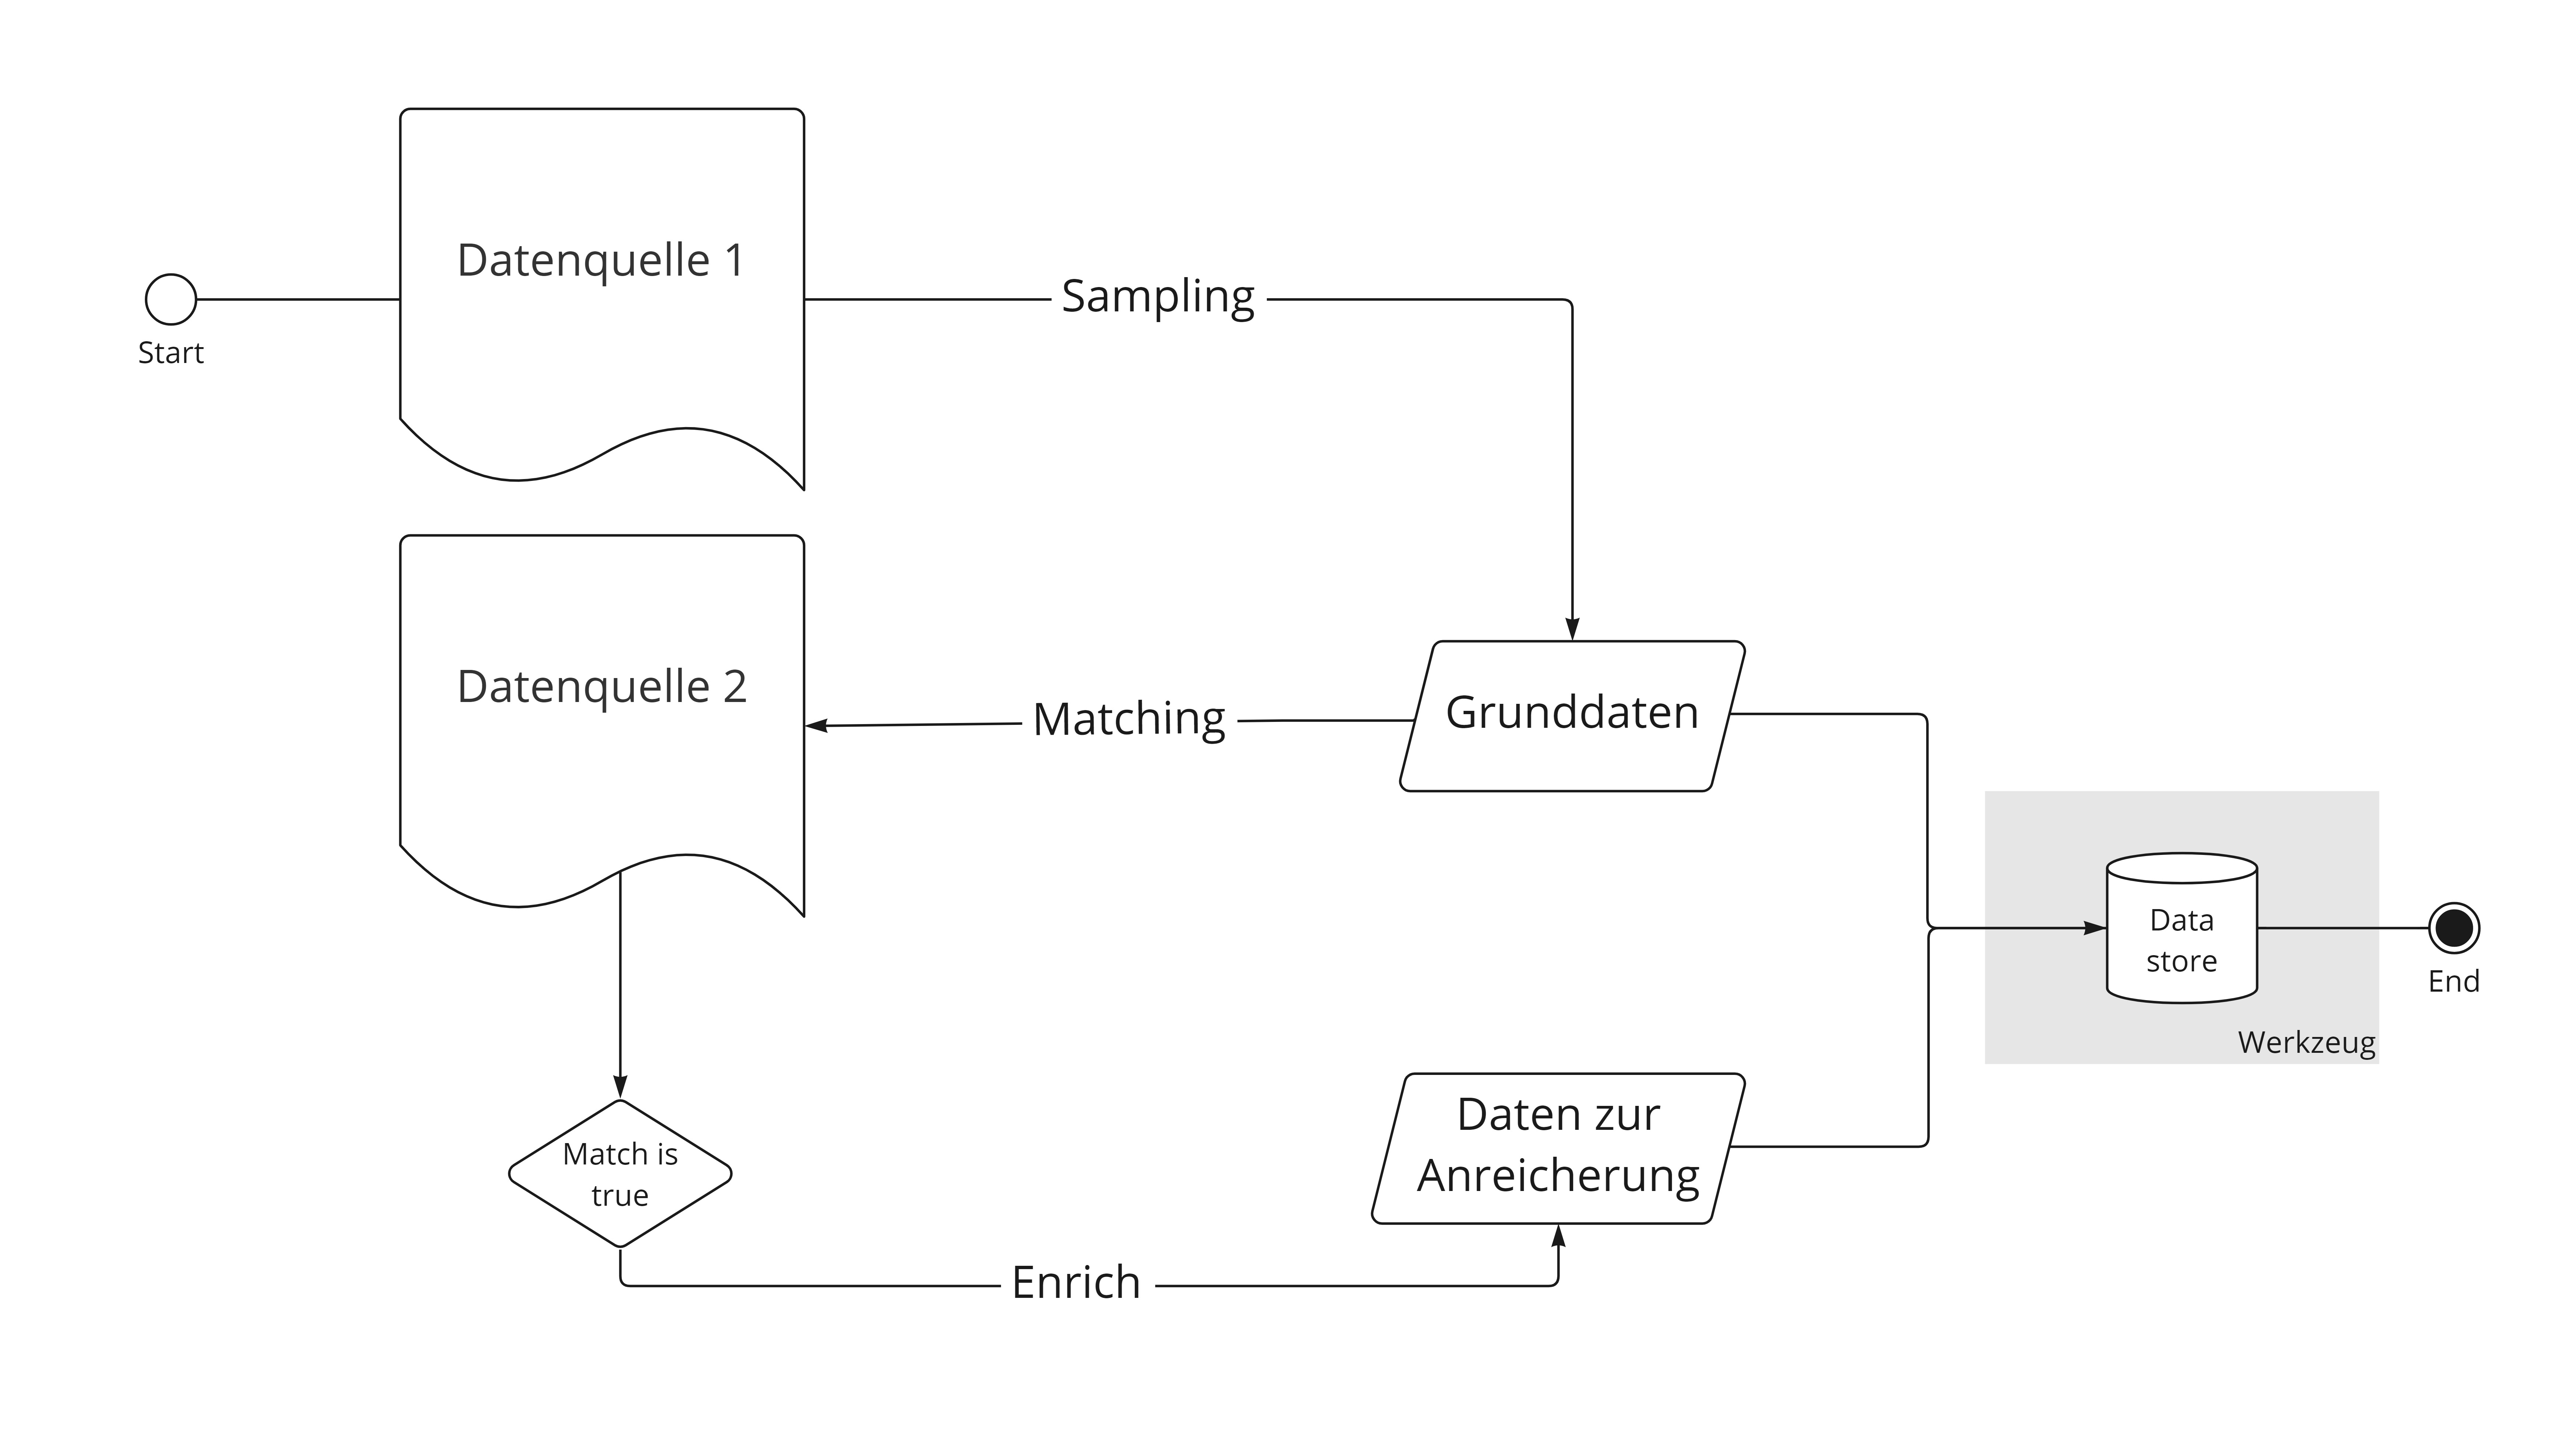
\includegraphics[width=\ScaleIfNeeded]{flowchart_data-collection}}
    \caption{Idealtypische Stichprobenziehung von Daten zu jüdischen Gewerbebetrieben.}
    \label{fig:x cubed graph}
\end{figure}

Nachteil der vereinfachten, groben Schematisierung ist, dass diese Detailinformationen nicht enthalten sind. Darüber hinaus fehlen die mit der Quellenlage einhergehenden Stichproben-Verzerrungen (Bias) der Studien, welche bisher überhaupt nicht kommuniziert werden:

\begin{itemize}
    \item Viele Hauptquellen setzen zeitlich erst mit den reichsweiten Gesetzen ab 1938 ein. Die frühe Phase der Vernichtung der jüdischen Gewerbetätigkeit bleibt somit unterrepräsentiert, weil schlichtweg Daten dazu fehlen.
    \item Bei der Verwendung von überwiegend Wiedergutmachungsakten, insbesondere aus Rückerstattungsverfahren wie in Hamburg, liegt der Schwerpunkt automatisch auf den größeren Unternehmensverkäufen und den ehemaligen Eigentümern, die den Nationalsozialismus meist durch Emigration überlebt haben. Liquidationen bleiben in diesem Ansatz unterrepräsentiert sowie der komplette Ostteil Deutschlands, da hier die Wiedergutmachung erst in den 90er Jahren mit dem Ende der DDR teilweise einsetzte.
    \item In Berlin wiederum liegt der Fokus mit der ZHRB auf den handelsregisterlich eingetragenen Firmen und damit auf mittelständischen Gewerbebetrieben, wodurch vor allem Kleinstunternehmen unterrepräsentiert bleiben. Außerdem liegt der Schwerpunkt auf Liquidationen, da das Handelsregister Besitzübernahmen nicht abbildet.
\end{itemize}

Es wird deutlich, dass geschichtswissenschaftliche Datenerhebungsmethoden aufgrund der historischen Quellengrundlage nicht analog zu den naturwissenschaftlichen Methoden standardisiert werden können. Es ist die Lückenhaftigkeit und es sind die Fehlstellen in der historischen Forschung, die eine adäquate Abbildung auf ein festes Schema zu einer spezifischen Herausforderung im Fach machen. Daher stellt sich insbesondere auch die Frage, welche Notwendigkeit Standardisierung hier besitzt. Es wäre genauer zu untersuchen, was der Mehrwert davon für die historische Forschung wäre oder ob zum Zwecke der methodischen Transparenz und Nachvollziehbarkeit eine rein textuelle Beschreibung oder Dokumentation zum Beispiel in Form einer Readme-Datei ausreicht. Tatsache ist, dass die Ausführungen zur Erhebung in die einzelnen Lokalstudien bisher unterschiedlich ausfallen und entscheidenden Informationen zum Verständnis der Forschungsdaten ganz fehlen. Auch im Sinne der Nachnutzbarkeit von historischen Forschungsdaten ist also die offene Frage, welche Informationen zur Methodik überhaupt benötigt werden.

\subsection{Problem \textit{Jüdischer} Gewerbebetrieb}

Da Untersuchungsgegenstand aller Lokalstudien ,,Jüdische Gewerbebetriebe'' oder ,,Jüdische Unternehmen'' sind, wurde folglich Daten zu jüdischen Gewerbebetrieben erfasst. Hieraus ergibt sich eine grundlegende methodische Schwierigkeit: Da die Konfessionszugehörigkeit bezüglich eines Gewerbebetriebs oder Unternehmens schlichtweg unlogisch ist, ist der Begiff alleine ohne Kontext unbrauchbar. Dieses Problem wird von dem meisten Studien reflektiert und betont, dass es sich hierbei um eine antisemitische Zuschreibung und Konstruktion handelte. Diese Kennzeichnung und Diffamierung diente den Nationalsozialisten als Instrument für die weiteren Verfolgungspraktiken. Zur einfacheren Handhabung wurde der Begriff als Quellenbegriff jedoch von allen Studien beibehalten. Hierbei fallen zwei unterschiedliche Verwendungen auf: 

\begin{itemize}
    \item Der Begriff ,,jüdischer Gewerbebetrieb'' wird ausschließlich auf die jüdischen Besitzer*innnen bezogen und angewandt.\footnote{Vgl. Janetzko 2012, S. 18.} Damit wird jedoch das methodische Problem nicht aufgelöst, sondern verlagert sich auf den Begriff ,,jüdische Person'' oder ,,Jude/ Jüdin'', bei dem es sich ebenfalls um eine rassistische Zuschreibung handelte und nichts mit dem Selbstverständnis der Betroffenen zu tun hatte.\footnote{Das wird in der Studie zu Hamburg auch ausführlich reflektiert. Vgl. Bajohr 1997, S. 9.} Darüber hinaus werden in dieser Verwendung weitere Verfolgungskontexte vernachlässigt. So war es in der frühen Phase der Verfolgung durchaus möglich, dass Gewerbebetriebe als jüdisch diffamiert wurden, die zum Beispiel einen hohen Anteil jüdischer Mitarbeiter*innen aufwiesen, deren Besitzer aber selbst nach der nationalsozialistischen Ideologie nichtjüdisch waren.\footnote{An diesem Beispiel zeigt sich überdies die in Wechselbeziehung stehenden Teilprozesse der Verdrängung der Juden aus dem Berufsleben und der Vernichtung der jüdischen Gewerbetätig deutlich.}
    \item Der Begriff ,,jüdischer Gewerbebetrieb'' wird mit ,,als jüdisch betrachtet/ verfolgt'' übersetzt. In dieser Verwendung ist die jüdische Eigentümerschaft eines Gewerbebetriebs zunächst unerheblich, das heißt sie wird nicht vorausgesetzt, sondern es werden alle Gewerbebetriebe erfasst, die im nationalsozialistischen Kontext diffamiert wurden. Damit wird einerseits der Konstruktioncharakter des Begriff hervorgehoben und andererseits dem Umstand Rechnung getragen, dass die rassistischen Zuschreibungen grundsätzlich jeglicher rationalen Begründung entbehrten und aus diesem Grund willkürlich erfolgen konnten.
\end{itemize}

Auch wenn in allen Studien der selbe Untersuchungsgegenstand genannt wird, so zeigt sich erst in der konkreten Verwendung, dass dieser unterschiedlich ausgedehnt werden konnte, weil der Begriff an sich nicht widerspruchsfrei ist. Aus forschungsethischer Perspektive ist zudem problematisch, dass ein rassistisch konnotierter Begriff in der wissenschaftlichen Forschung beibehalten wird. Wichtig wäre, sich im Forschungsfeld auf eine einheitliche Verwendung zu einigen, denn bisher werden Jüdische Gewerbebetrieben unterschiedlich erhoben. Hierzu wird keine abschließende Entscheidung getroffen, da dies in einem Diskurs im Forschungsfeld gemeinsam entschieden werden sollte. Um dafür den Anstoß zu geben und um insbesondere auch die forschungsethischen Implikationen kritisch zu reflektieren, wurde im erstellten Wikidata-Projekt\footnote{Zum Wikidata-Projekt siehe Kapitel 4.3.} der \textit{Wikidata talk} ,,How do we use and model ,Jüdischer Gewerbebetrieb'?'' mit der Disskussionsfunktion angelegt und zwei Vorschläge unterbreitet (Abbildung ): 

\begin{itemize}
    \item ,,Jüdischer Gewerbebetrieb'' wird als eigenes Item angelegt und mit Statements angereichert, die die nationalsozialistische Herkunft deutlich machen. Da in Wikidata Items von jedem/ jeder ohne Einschränkung angelegt werden können, wäre diese Lösung schnell umsetzbar. Bei der Frage mit welcher Eigenschaft (Property) das Item als Value auf einen Gewerbebetrieb abgebildet werden soll, lohnt abermals ein Blick auf benachbarte Wikidata-Projekte. Im Projekt \textit{Wikidata:WikiProject Victims of National Socialism} wurde 2020 die Verwendung des Begriffs ,,Holocaust-Opfer'' diskutiert.\footnote{Wikidata Talk:Q2763 (2020), Modeling of holocaust victim, URL: \url{https://www.wikidata.org/w/index.php?title=Talk:Q2763&oldid=1392179230}}. Da in der Wikidata Konvention ist, Personen so neutral wie möglich zu beschreiben und Zuschreibungen von außen mit entsprechenden Aussagen kenntlich zu machen, hat man sich im Wikidata-Projekt darauf geeinigt, den Begriff nunmehr zusammen mit ,,Subjekt fungiert als (P2868) Opfer des Holocaust (Q5883980)'' zu verwenden und nicht mehr als ,,ist ein(e) (P31) Holocaust-Opfer (Q5883980)''.\footnote{Siehe zum Beispiel Wikidata-Item Anne Frank (Q4583), URL: \url{https://www.wikidata.org/w/index.php?title=Q4583&oldid=1645273699}.} Diese Verwendung kann für Gewerbebetriebe übernommen werden. Zwar geht es hier ausdrücklich nicht um Personen. Da aber die Verwendung ,,ist ein(e) (P31) Jüdischer Gewerbebetrieb (Q???)'' - wie gezeigt wurde - unlogisch wäre, bietet sich ,,Subjekt fungiert als (P2868) Jüdischer Gewerbebetrieb (Q???)'' an.
    \item Statt als Item kann ,,Jüdischer Gewerbebetrieb'' auch als Property ,,als jüdisch betrachtet/ verfolgt (P???)'' oder ähnlich modelliert werden.\footnote{Dieser Ansatz wurde vom Berliner Forschungsprojekt umgesetzt.} Da diese Eigenschaft bisher noch nicht existiert, wäre diese Umsetzung etwas langwieriger, da Eigenschaften in der Wikidata nicht von jedem/jeder erstellt werden, sondern zunächst vorgeschlagen werden müssen.\footnote{Wikidata:Eigenschaften vorschlagen (2022), URL (stable): \url{https://www.wikidata.org/w/index.php?title=Wikidata:Property_proposal/de&oldid=1624532274}.} Nach einer öffentlichen Debatte entscheidet eine berechtigte Administratoren-Gruppe der Wikidata, ob die Property neu aufgenommen wird oder ob Alternativ-Eigenschaften zur Verfügung stehen. Mit diesem Verfahren sollen Redundanzen und Widersprüchlichkeiten verhindert werden. Es dient zur Qualitätskontrolle der Wikidata. Daher ist es möglich, dass für das Forschungsfeld notwendige Eigenschaften für die Wikidata insgesamt nicht die Relevanz besitzen und aus diesem Grund abgelehnt werden können. Wie liberal oder konservativ die Wikidata-Politik hier ist, müsste erprobt werden.      
\end{itemize} 

\begin{figure}[h]
    \centering
    \frame{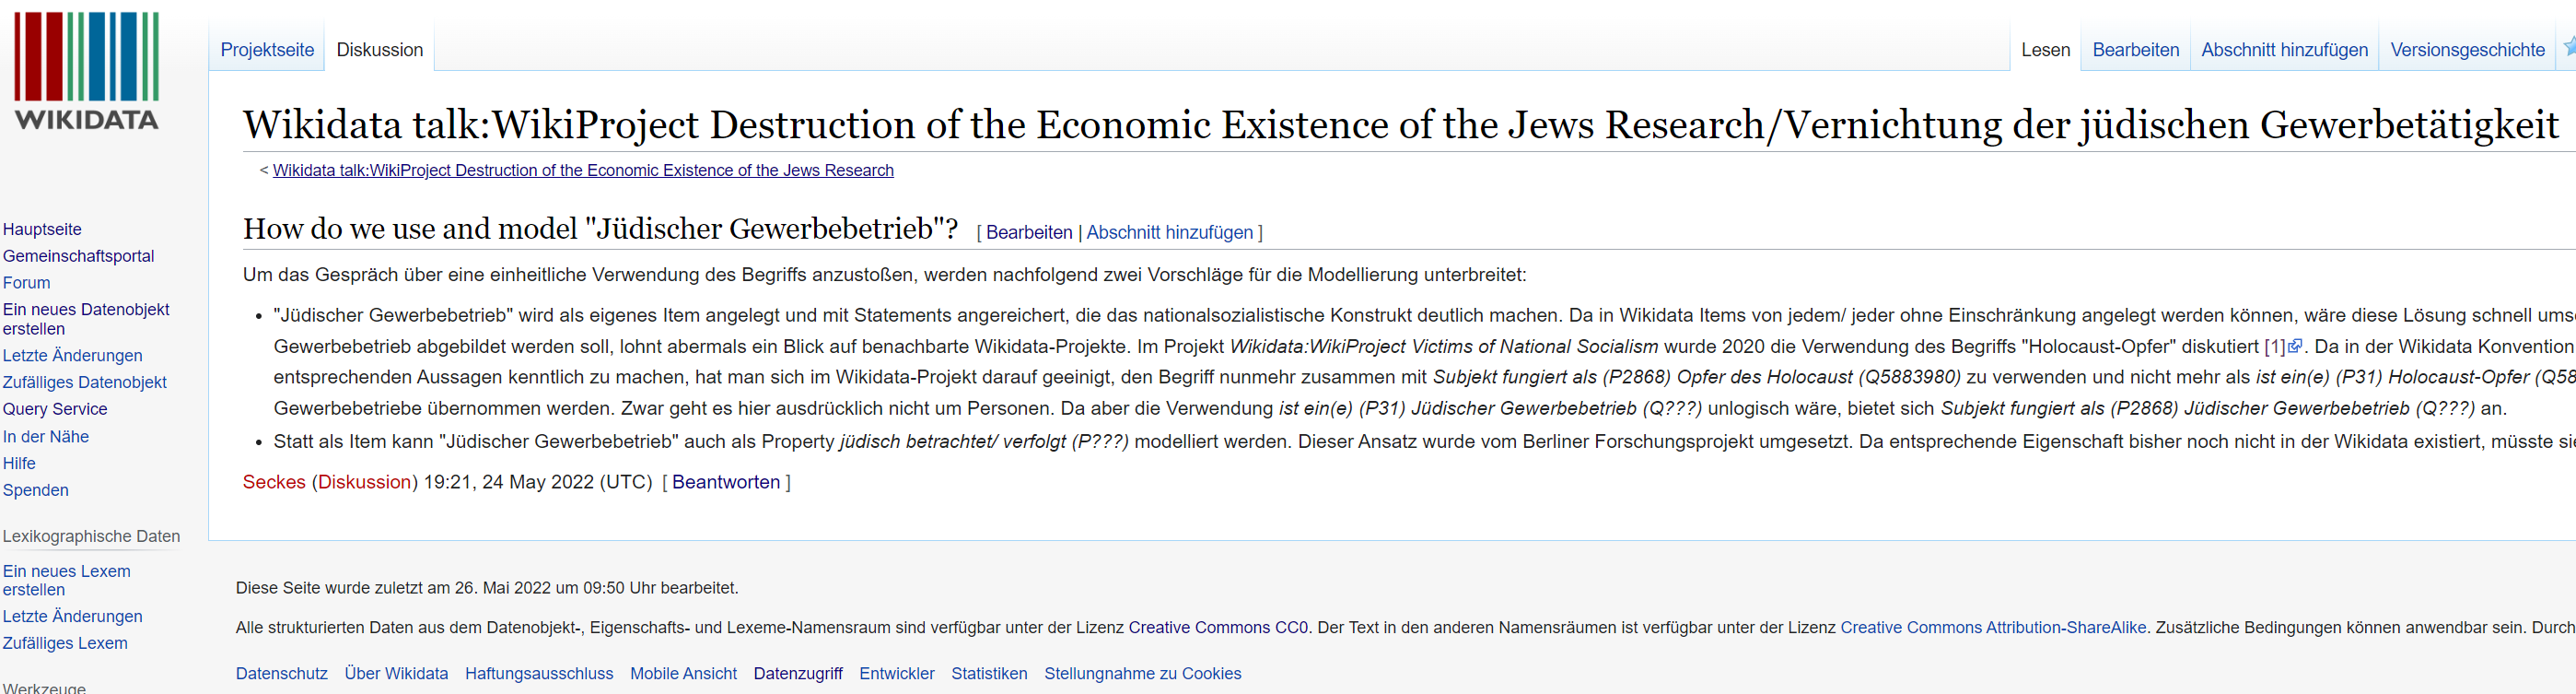
\includegraphics[width=\ScaleIfNeeded]{wikidata-discussion-jued-gewerbebetrieb}}
    \caption{Diskussionsseite zur Frage, wie "Jüdischer Gewerbebetrieb" verwendet und modelliert werden soll.}
    \label{fig:x cubed graph}
\end{figure}

\section{Aufbereitung}

\begin{quote}
    Also ich denke, die sitzen alle auf irgendwelchen Excellisten oder wenn das ältere Forschungsprojekte sind, Herr Bajohr weiß ich nicht, ob der schon Excel genutzt hat für sein Hamburg-Buch oder ob der noch Karteikarten hatte.\footnote{Interview B3\_Transkript, Pos. 79.}
\end{quote}

Um eine valide Datengrundlage für die Analyse zu erhalten, werden die erhobenen Rohdaten vorab aufbereitet. Damit erfolgt erstmalig eine Verarbeitung der Daten, denn der Operationalisierung der Forschungsfragen entsprechend werden die Daten ausgewählt, strukturiert erfasst und bereinigt. In der historischen Forschung liegt die Situation vor, dass die Rohdaten im Quellenmaterial bereits vorliegen, sich aber mitunter über viele Quellen verteilen. Daher muss festgelegt werden, erstens welche Informationen aus den Quellen extrahiert werden sowie zweitens, mit welchem Werkzeug diese strukturiert und organisiert werden sollen. Dieser Prozess der Forschungsdaten-Genese ist bisher im Forschungsfeld weitestgehend unsichtbar und findet lediglich in den Studien zu Berlin und Frankfurt am Main nachträglich in den Publikationen Erwähnung.\footnote{Vgl. Kreutzmüller 2012, S. 38f., Nietzel 2012, S. 17.}. In beiden Projekten kamen ,,Datenbanken'' zum Einsatz, die anhand der Interviews als Microsoft Access-Datenbanken der Version 2007 spezifiziert werden konnten.\footnote{Vgl. Interview B2\_Transkript, Pos. 27.} Da es sich hierbei um eine Anwendung handelt, deren Datenorganisation auf relationalen Tabellen beruht, braucht es als Basis vorab ein Datenmodell, visualisiert zum Beispiel anhand eines Entity-Relationship-Diagramms (ERD) mit einer Beschreibung der darin verwendeten Elemente. Dieses ist für beide Studien allerdings nicht verfügbar. Damit ist eine Beurteilung der Daten hinsichtlich ihrer Verarbeitung bisher nicht möglich. Ziel von offenem Forschungsdatenmanagement ist es, die bisher unsichtbare Phase der Aufbereitung durch kollaborative Zusammenarbeit im Forschungsfeld transparenter zu gestalten. 

Zu diesem Zweck wurde in Wikidata das Projekt \textit{Wikidata:WikiProject Destruction of the Economic Existence of the Jews Research} erstellt (Abbildung 4.3.).\footnote{URL: \url{https://www.wikidata.org/wiki/Wikidata:WikiProject_Destruction_of_the_Economic_Existence_of_the_Jews_Research}.} Dieses besitzt grob drei Funktionen: Erstens können beliebig viele Seiten mithilfe von standardisierten Templates hierarchisch im Projekt angelegt werden (Pages und Subpages).\footnote{Siehe URL: \url{https://www.mediawiki.org/wiki/Help:Templates} (letzter Zugriff am 24.05.2022).} Diese bieten die Möglichkeit, die in Kapitel 3 methodisch aufgegriffene Taxonomie und damit die unterschiedlichen Zugänge im Forschungsfeld funktional umzusetzen. Auf der Hauptseite (Home) wurden bereits Hintergrundinformatioen zum Projekt sowie zu dessen Zielen hinzugefügt. Dort ist auch erwähnt, dass diese Arbeit nur den Ausgangspunkt bildet und von hier aus sukzessive die angrenzenden Untersuchungsbereiche integriert werden können. Außerdem findet sich hier die nicht unwichtige Information, dass die Taxonomie im Forschungsfeld dem Systematisierungversuch von Nietzel aus dem Jahr 2009 entlehnt ist.\footnote{Siehe Kapitel 3.2.1.}

\begin{figure}[h]
    \centering
    \frame{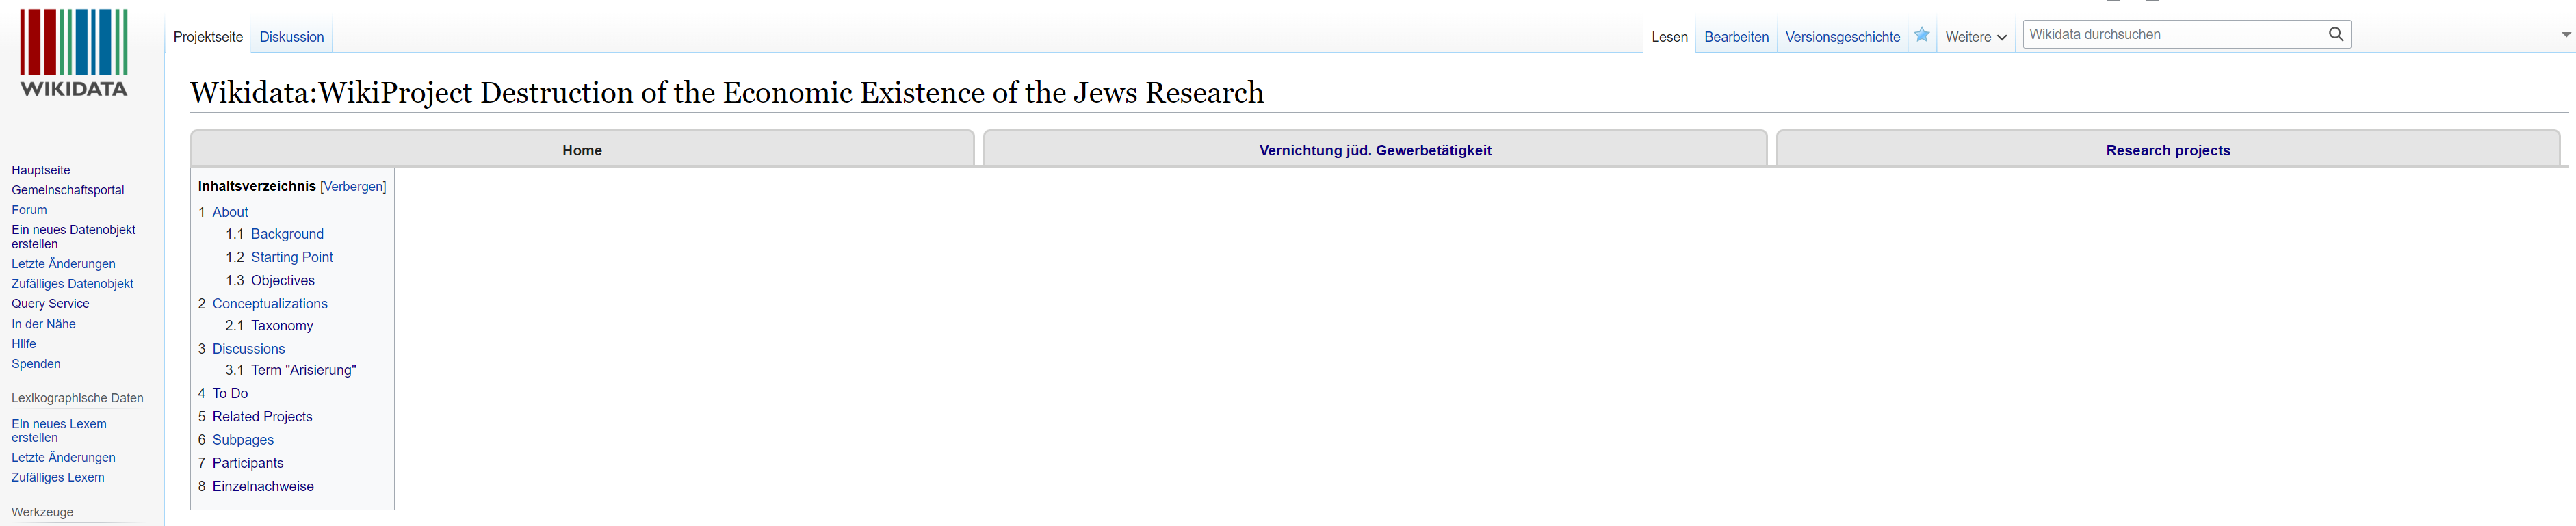
\includegraphics[width=\ScaleIfNeeded]{wikidata-project_tabs}}
    \caption{Wikidata:WikiProject Destruction of the Economic Existence of the Jews Research mit den in Tabs angelegten Subpages.}
    \label{fig:x cubed graph}
\end{figure}

Die bisherige Implementierung versteht sich explizit als Vorschlag, um eine Ausgangsbasis zu haben, von der aus Anpassungen und Weiterentwicklungen möglich werden. Um später in den gemeinsamen Austausch zu treten und Änderungen vorzunehmen, kann hierfür die zweite grundlegende Funktion der Diskussionseiten genutzt werden. Schließlich gibt es mit der Versionierung (,,Versionsgeschichte'') eine Kontrollfunktion, mit der sich alle Bearbeitungen zurückverfolgen und gegebenfalls auf einen früheren Stand zurücksetzen lassen.\footnote{URL: \url{https://www.wikidata.org/w/index.php?title=Wikidata:WikiProject_Destruction_of_the_Economic_Existence_of_the_Jews_Research&action=history} (letzter Zugriff am 24.05.2022).} Ingesamt bietet das Wikidata-Projekt damit die Möglichkeit des kollaborativen Austauschs und der gemeinsamen Strategieentwicklung im Forschungsfeld. Erstmals können Methodiken und Konzepte im Forschungsfeld diskutiert sowie in Bezug auf die in der Arbeit betrachteten Forschungsdaten ein allgemeingültiger Leitfaden zur Erfassung jüdischer Gewerbebetriebe entwickelt werden. Thematisch ist das Wikidata-Projekt in die Kategorien \textit{History WikiProjects} und \textit{Research WikiProjects} eingeordnet.\footnote{Siehe Wikidata:WikiProjekte, URL: \url{https://www.wikidata.org/wiki/Wikidata:WikiProjects/de} (letzter Zugriff am 24.05.2022).} Hier zeigt sich darüber hinaus, dass benachbarte Forschungsfelder zum Nationalsozialismus und zum Holocaust bereits mit eigenen Projekten vertreten sind, womit sich Anknüpfungspunkte über das Forschungsfeld hinaus ergeben.\footnote{Siehe WikiProject WWII, URL: \url{https://www.wikidata.org/wiki/Wikidata:WikiProject\_WWII}; WikiProject NS Perpetrator Research, URL: \url{https://www.wikidata.org/wiki/Wikidata:WikiProject\_NS\_Perpetrator\_Research}; WikiProject Victims of National Socialism, URL: \url{https://www.wikidata.org/wiki/Wikidata:WikiProject\_Victims\_of\_National\_Socialism}; WikiProject NS-Täterforschung, URL: \url{https://www.wikidata.org/wiki/Wikidata:WikiProject\_NS-Täterforschung}; Wikidata:WikiProject Nuremberg Trials, URL: \url{https://www.wikidata.org/wiki/Wikidata:WikiProject\_Nuremberg\_Trials} (alle letzter Zugriff am 24.05.2022).} 

\subsection{Zusammenführung der Quellen}

\paragraph{Datenmodell} Beim Zusammenführen der Quellen wurden die ausgewählten verteilten Informationen als strukturierte Daten zentral in Excel oder Access gespeichert. Auch wenn es in den Interviews von keinem Befragten bewusst formuliert wurde, so haben alle zur ,,Handhabbarmachung der Informationen''\footnote{Kreutzmüller 2012, S. 38.} eine \textit{Modellierung} von den zu erfassenden Daten vorgenommen. Bei diesem Vorgang wird ein eindeutig definierter realer Ausschnitt auf ein Modell abgebildet und die enthaltenen Konzepte operationalisiert. Aus den Interviews geht außerdem hervor, dass ein Datenmodell vorab nicht fest fixiert war, sondern dieses parallel zur Datenerfassung entstand und erweitert wurde.\footnote{Interview B1\_Transkript, Pos. 3, B2\_Transkript, Pos. 31 und Interview B1\_Transkript, Pos. 75.} Daraus ergeben sich zwei Anforderungen an offenes Forschungsdatenmanagement: Kollaborative Zusammenarbeit zwischen den Projekten kann nur funktionieren, wenn man sich auf eine Terminologie und auf ein Schema einigt. Es müssen folglich erstens die vielen unterschiedlichen Modelle und Begriffe der einzelnen Studien für eine gemeinsame Nutzung kompatibel gemacht werden. Da aufgrund der besonderen Überlieferungsstruktur ein statisches Modell vorab nicht feststeht, muss dieses zweitens dynamisch und skalierbar sein.

Anhand der für die Arbeit zu Verfügung gestellten Daten aus Berlin, Mannheim und Krefeld sowie mithilfe der Interviews wurde zunächst versucht, eine begriffliche Kontrolle im Untersuchungsfeld zur Vernichtung der jüdischen Gewerbetätigkeit im NS zu erhalten. Hierbei wurde sich der Methodik der Dokumentbeschreibungssprachen aus den Bibliotheks-, Dokumentations- und Informationswissenschaften bedient, mit der Fachgebiete mittels Thesauri oder Klassifikationen hierarchisch geordnet und inhaltlich erschlossen werden (Sacherschließung).\footnote{Siehe Gernot Wersig: Thesaurus-Leitfaden. Eine Einführung in das Thesaurus-Prinzip in Theorie und Praxis, Berlin, Boston 2016, doi:10.1515/9783111412719.} In diesem Sinne wird das Untersuchungsfeld als eigenes Begriffssystem verstanden, mittels dessen es sich inhaltlich beschreiben lässt.\footnote{Der erstellte Thesaurus als Anhang ... beigefügt.} Auf diese Weise konnte nicht nur eine Übersicht über die wesentlichen historischen Informationen im Untersuchungsfeld erstellt werden, sondern es zeigte sich mit dieser Methode auch, dass es zum einen Mehrdeutigkeiten bei der Bezeichnung von Sachverhalten gibt (Synonymproblem) und zum anderen Unklarheiten bestehen, wie Begriffe angewandt werden sollen.\footnote{Ebd., S. 47-51.} Für das Synonymproblem können Äquivalenzklassen vorgeschlagen werden.\footnote{Im Modell in den einzelnen Kästchen fett hervorgehoben} Die unklaren Begriffe müssen in dieser Arbeit offen bleiben, da abschließend deren globale Relevanz für das Forschungsfeld nicht bestimmt (z.B. Insolvenz)\footnote{Die Geschäftsauflösung bzw. Insolvenz wurde nur in der Krefelder Studie untersucht.} oder ihre Ambiguität (z.B. Geschäftsaufgabe) nicht aufgelöst werden konnte. 

Das feine Begriffssystem\footnote{Im Modell grau hinterlegt} wurde grob abstrahiert, sodass die generischen Begriffe auf der ersten Ebene eine Top-Level-Ontologie ergeben, die Studien-unabhängig auf alle Forschungsdaten im Forschungsfeld und darüber hinaus angewandt werden kann.\footnote{Siehe zu Top-Level-Ontologie Rehbein, Ontologien, 2017, S. 162-174.} Auf diese Weise kann das Datenmodell kompatibel und interoperabel gehalten werden, in der Konsequenz also zukünftig auch an andere Forschungsfelder anschließen.

Das generische Metadatenschema wurde im nächsten Schritt in das Wikidata-Projekt integriert, welches somit eine Strukturierung der Daten grob vorgibt (Abbildung 4.5.). 

\begin{figure}[h]
    \centering
    \frame{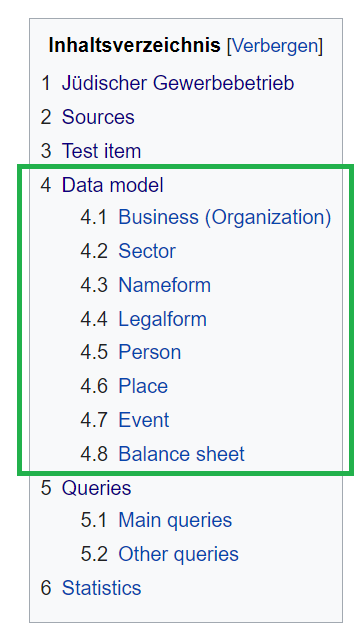
\includegraphics[scale=0.6]{wikidata-data-model-generic}}
    \caption{Integration des Metadatenschemas in Wikidata.}
    \label{fig:x cubed graph}
\end{figure}

Am Beispiel des Berliner Gewerbebetriebs ,,Gorbatschow Liköre F. Kramer \& Co'', welches 1938 vom Eigentümer Josef Kramer verkauft werden musste, wurde ein erster Entwurf für das präzise Datenmodell in Wikidata erstellt.\footnote{Das Modell ist als Anhang ... beigefügt.} Analog zur Modellierung der Forschungsprojekte wurden vorhandene Items und Properties nachgenutzt. Wo dies nicht möglich war, sind die Entities farblich markiert. Der Entwurf wurde anschließend im Wikidata-Projekt dokumentiert (Abbildung 4.6. Siehe auch Wikidata-Projekt, URL (stable): \url{https://www.wikidata.org/w/index.php?title=Wikidata:WikiProject\_Destruction\_of\_the\_Economic\_Existence\_of\_the\_Jews\_Research/Vernichtung\_der\_jüdischen\_Gewerbetätigkeit&oldid=1648462059}.).   

\begin{figure}[h]
    \centering
    \frame{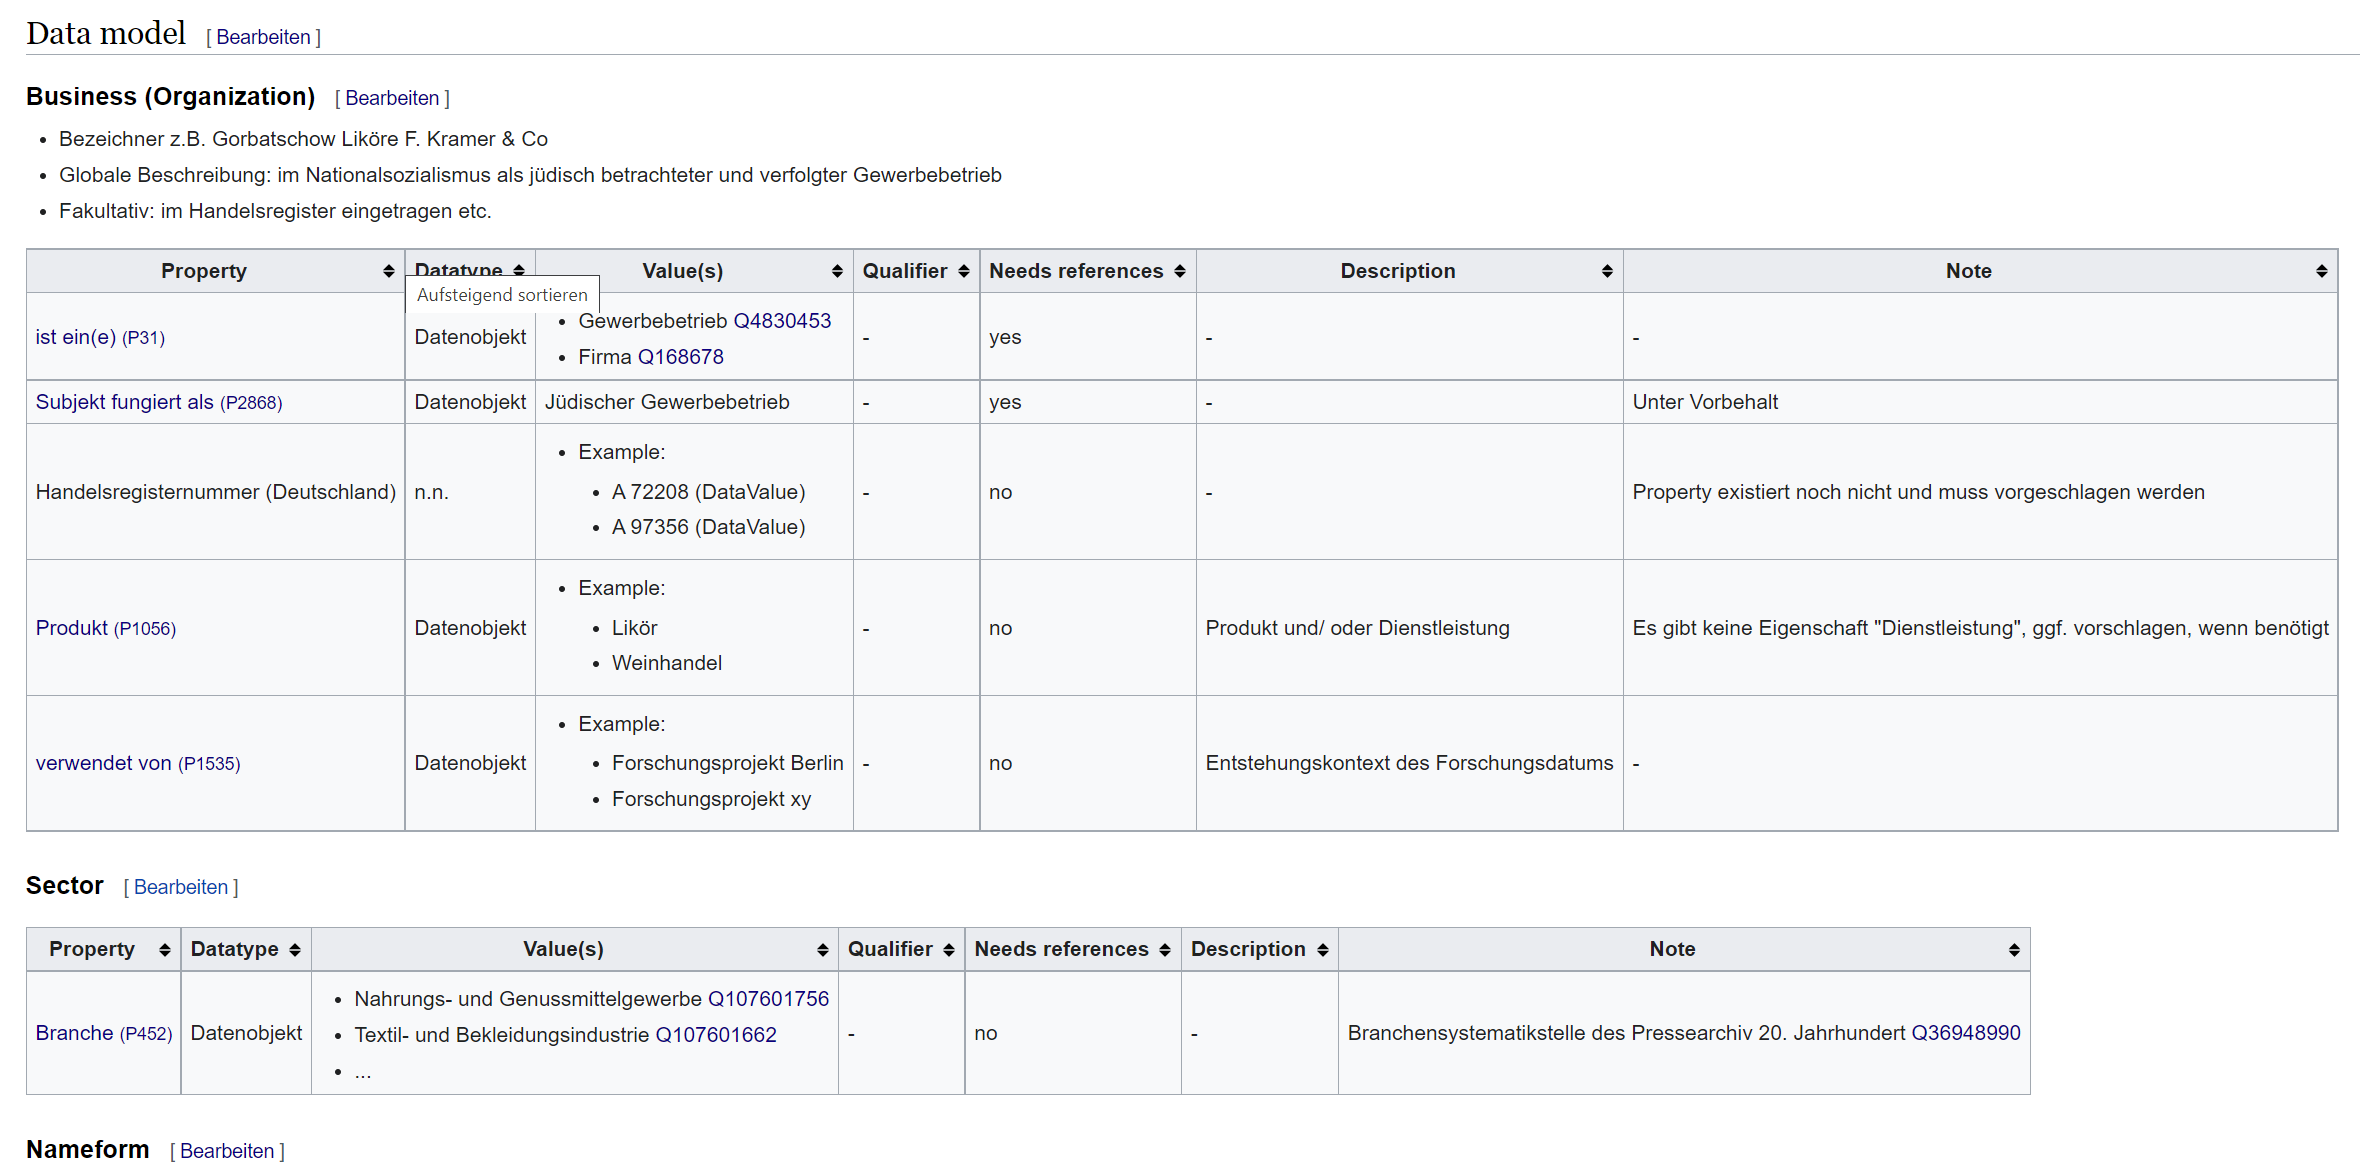
\includegraphics[width=\ScaleIfNeeded]{wikidata-data-model}}
    \caption{Beschreibung der Statements zu den einzelnen Entities.}
    \label{fig:x cubed graph}
\end{figure}

Hier kann das Datenmodell zur Beschreibung jüdischer Gewerbebetriebe kollaborativ angepasst und weiterentwickelt werden. In der Tabelle in Abbildung 4.6 stellt jede Zeile eine Aussage zu einer Entität dar (im Bild Gewerbebetrieb und Branche). In dieser können neben der Statements außerdem Verwendungsregeln und detaillierte Beschreibungen festgehalten werden. Das aktuelle prototypische Datenmodell versteht sich lediglich als Vorschlag und soll in erster Linie den Anstoß für weitere Diskussionen geben. Denn insbesondere die Frage nach der Modellierung der Forschungsdaten wird im Forschungsfeld bisher nicht systematisch bearbeitet. Aber schon in dieser frühen Phase ergeben sich Pfadabhängigkeiten, die Einfluss auf die anschließende Datenanalyse haben. Dies kann an einem Beispiel veranschaulicht werden: Wenn zu einem Gewerbebetrieb nur eine Adresse strukturiert erfasst wird (1:1 Kardinalität), können (überregionale) Umzüge später nicht mehr untersucht werden. In Berlin gab es in der Access-Datenbank nur Felder für eine Adresse pro Gewerbebetrieb. Weitere Adressen wurden unstrukturiert in sogenannten Freitextfeldern erfasst. Damit war und ist es nur schwer möglich, sich der Untersuchung von Ausweichsbewegungen - was in Berlin nur auf qualitativer Ebene geschah - quantitativ zu nähern.\footnote{siehe Kreutzmüller 2012, S. 310-310 (Kap. Umzug).} Wikidata mit dem dahinter stehenden Linked Data-Konzept bietet demgegenüber den entscheidenden Vorteil, dass ausschließlich strukturierte Daten in Subjekt-Prädikat-Objekt-Ausdrücken erfasst sowie neue Properties und Items dynamisch ergänzt werden können. Eine aufwändige Anpassung des Datenmodells entfällt dadurch. Die Einschränkung ist jedoch, dass erfasste Daten zu Jüdischen Gewerbebetrieben nicht gegen das Modell geprüft werden können. Das bedeutet, dass Daten auf der technischen Ebene auch dann gültig wären, wenn diese vollkommen anders erfasst würden. Damit ist eine Kontrolle über die Gültigkeit von Daten zu Jüdischen Gewerbebetrieben zum jetzigen Zeitpunkt nicht gegeben. Wikidata bietet aber mit dem Ziel der weiteren Qualitätssicherung die Erstellung von \textit{EntitySchemas} an (Abbildung 4.7).\footnote{Siehe Wikidata Schemas, URL: \url{https://www.wikidata.org/wiki/Wikidata:Schemas}. Siehe zum Beispiel das Entity Schema zu Mensch (E10), URL: \url{https://www.wikidata.org/wiki/EntitySchema:E10} (alle letzter Zugriff am 27.05.2022).} Damit ließe sich ein verbindliches Schema zur Erfassung von Jüdischen Gewerbebetrieben definieren. Dies ist jedoch erst dann sinnvoll, wenn ein gemeinsamer Grundstamm an Aussagen im Forschungsfeld feststeht.

\begin{figure}[h]
    \centering
    \frame{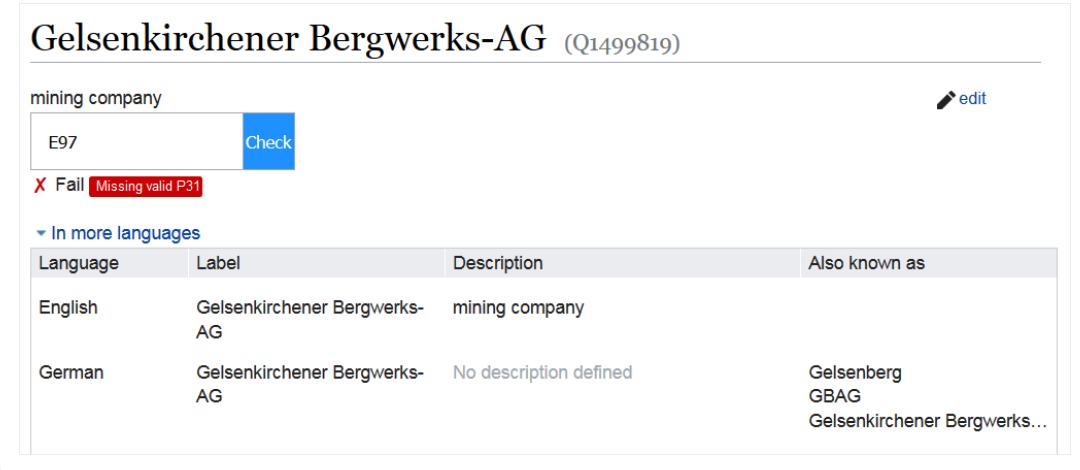
\includegraphics[scale=0.7]{wikidata-entity-schema}}
    \caption{Mithilfe von EntitySchemas können Daten gegen ein fest definiertes Schema auf ihre Gültigkeit hin geprüft werden.}
    \label{fig:x cubed graph}
\end{figure}

\paragraph{Personenbezogene Daten}

Auch wenn die Daten zu jüdischen Gewerbebetrieben größtenteils als ethisch unbedenklich eingestuft wurden\footnote{Vgl. Kapitel 3.5.}, gibt es mit den Unternehmenseigentümern personenbezogene Daten, die besondere forschungsethische Fragen aufwerfen, wenn sie in Open Data verfügbar sind. Zu beachten ist, dass es sich in der Regel nicht um Personen des öffentlichen Interesses handelt, was eine detaillierte Veröffentlichung bibliografischer Daten rechtfertigen würde. Das bedeutet, dass der Eigentümer Josef Kramer von Gorbatschow Liköre F. Kramer \& Co nicht mit Anne Frank\footnote{Wikidata-Item Anne Frank (Q4583), URL: \url{https://www.wikidata.org/wiki/Q4583}.} oder der Holocaust-Überlebenden und Aktivistin Margot Friedländer\footnote{Wikidata-Item Margot Friedländer (Q1895371), URL: \url{https://www.wikidata.org/wiki/Q1895371}.} gleichzusetzen ist. Gerade auch die Fälle, wo ehemalige Inhaber den Holocaust durch Emigration überlebt haben und nach 1945 einen Antrag auf Rückerstattung stellten, können rechtliche Einwände gegen eine Veröffentlichung von detaillierten personenbezogenen Daten sprechen.\footnote{Vgl. Kapitel 3.5.} Anders als bisher im Forschungsfeld braucht offenes Forschungdatenmanagent in Wikidata hier ein gemeinsames Vorgehen sowie eine klare und nachvollziehbare Strategie, die den verantwortungsvollen Umgang mit diesen sensiblen Daten sicherstellt. 

Hierzu wird folgende Empfehlung gemacht: Generell sollte das grundlose Sammeln personenbezogener Daten vermieden werden. Das bedeutet, auch wenn sie in den Quellen vorhanden sind, aber nicht der Bearbeitung von Forschungsfragen direkt dienen, werden sie nicht in Wikidata aufgenommen. Der Grundsatz ist, so wenig wie möglich personenbezogene Daten und so viel wie nötig zu erfassen. Sofern es also keine personenbezogenen Forschungsfragen gibt, werden lediglich Daten erfasst, die im Zusammenhang mit der unternehmerischen Tätigkeit stehen. Dies wurde am Beispiel der Gorbatschow Liköre F. Kramer \& Co für den Eigentümer Josef Kramer in Wikidata umgesetzt.\footnote{Wikidata-Item Josef Kramer (Q112135768), URL: \url{https://www.wikidata.org/wiki/Q112135768}.} Wenn wie in einigen Lokalstudien das Schicksal der Eigentümer nach der Besitzübernahme oder Liquidation statistisch untersucht werden soll\footnote{Siehe Bajohr 1998, S. 388 und Nietzel 2012, S. 121ff.}, werden hier nur die wesentlichen Informationen zu Emigration oder Deportation aufgenommen. Bei der Beschreibung des Verfolgungskontextes wird auf das bereits erwähnte WikiData-Projekt ,,Wikidata:WikiProject Victims of National Socialism'' zurückgegriffen. Demnach werden die Eigentümer*innen mit ,,Subjekt fungiert als (P2868) Holocaustüberlebender (Q12409870)'' bzw. ,,Subjekt fungiert als (P2868) Opfer des Holocaust (Q5883980)'' beschrieben. Für deren Schicksal werden die Aussagen ,,Schlüsselereignis (P793) ist ein(e) (P31) Holocaust-Gefangenentransport (Q61927259)'' bzw. ,,Schlüsselereignis (P793) ist ein(e) (P31) Auswanderung (Q187668)'' verwendet. Für den Fall, dass es weitere Informationen zu den Eigentümer*innen in externen öffentlichen Datenbanken gibt, die aber für die eigene Forschung nicht relevant sind, kann zur Datenvernetzung die eindeutige externe Personenkennung als Wikidata-Identifikator hinzugefügt werden (Abbildung 4.8).

\begin{figure}[h]
    \centering
    \frame{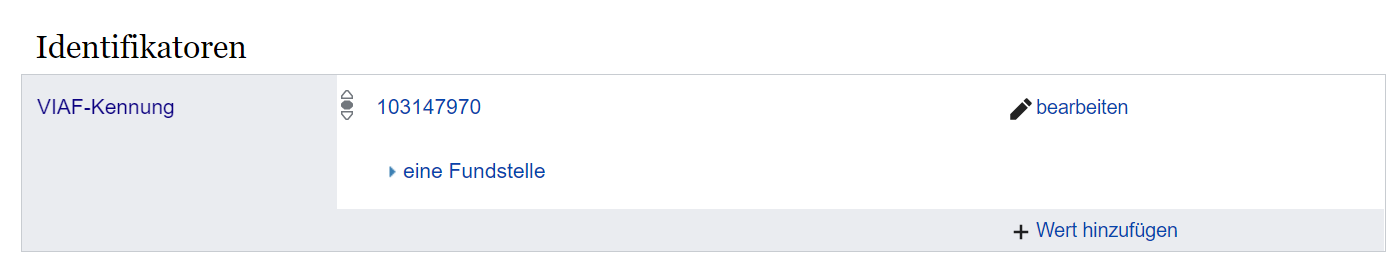
\includegraphics[width=\ScaleIfNeeded]{wikidata-idenficator}}
    \caption{VIAF-Kennung der Holocaustüberlebender und Aktivistin Eva Schloss als Wikidata-Identifikator im zugehörigen Wikidata-Item \url{https://www.wikidata.org/wiki/Q90250}.}
    \label{fig:x cubed graph}
\end{figure}

Aus forschungsethischer Sicht kann das in dieser Arbeit angelegte Wikidata-Projekt ein Forum sein, wo die Handhabung personenbezogener Daten diskutiert werden kann und wo allgemeingültige Grundsätze sowie Strategien festgehalten werden können.\footnote{Der Vorschlag aus dieser Arbeit wurde auf der Diskussionsseite im Wikidata-Projekt dokumentiert.} Damit wäre es über die Datenmodellierung hinaus eine Plattform, die wichtige Orientierung im Umgang mit sensiblen Daten im Forschungsfeld gibt vor allem auch für Forscher*innen, die sich gänzlich neu mit dem Thema befassen.

\paragraph{Quellennachweise}

Die Information, woher die Daten zu jüdischen Gewerbebetrieben kommen, stellt das vielleicht wichtigste Qualitätskriterium von offenem Forschungsdatenmanagement im Forschungsfeld dar.\footnote{Vgl. Interview B1\_Transkript, Pos. 139 und Interveiw B3\_Transkript, Pos. 73.} Insbesondere weil der Untersuchungsgegenstand ,,Jüdischer Gewerbebetrieb'', wie gezeigt worden ist, methodische Schwierigkeiten mit sich bringt, braucht es Nachweise, die diesen in den Quellen eindeutig belegen. Wikidata ist für diese Anforderung funktional besonders gut geeignet. Denn die globale Wissensdatenbank versteht sich ausdrücklich als sekundäre Datenbank und nicht als Primärquelle.\footnote{Vgl. Wikidata Hilfe:Belege, URL: \url{https://www.wikidata.org/wiki/Help:Sources/de} und Wikidata:Nachprüfbarkeit, URL: \url{https://www.wikidata.org/wiki/Wikidata:Verifiability/de} (alle letzter Zugriff am 28.05.2022).} Das bedeutet, dass jede Aussage in Wikidata grundsätzlich als Behauptung aufgefasst wird, die erst dann als valide gewertet wird, sobald sie durch Quellen- und Literaturangaben belegt ist. Um den hohen Anspruch der Nachprüfbarkeit erfüllen zu können, enthält das allgemeine Datenmodell der Wikidata neben der Items, Properties außerdem noch sogenannte Qualifier und References (Fundstellen), die jedem Aussagenwert (Value) eines Items beliebig oft hinzugefügt werden können.\footnote{Siehe Wikidata Help:Qualifikatoren, URL: \url{https://www.wikidata.org/wiki/Help:Qualifiers/de} und Wikidata:Tours/References, URL: \url{https://www.wikidata.org/w/index.php?title=Wikidata:Tours/References&oldid=1619471790} (alle letzter Zugriff am 28.05.2022).} Der Funktionsumfang der Wikidata geht hier also über das einfache Linked Data-Modell weit hinaus. Bei der Zitation und Erstellung von bibliografischen Items, orientiert sich Wikidata zudem an bewährten bibliografischen Metadatenstandards wie zum Beispiel \textit{Functional Requirements for Bibliographic Records} (FRBR) und verweist auf entsprechende Wikidata-Projekte, die sich auf die Modellierung bestimmer Quellengattungen spezialisiert haben.\footnote{Vgl. Wikidata Hilfe:Belege, ebd. Zu FRBR siehe IFLA Study Group on the Functional Requirements for Bibliographic Records, Susanne Oehlschläger: Funktionelle Anforderungen an bibliografische Datensätze. Abschlussbericht (2006), in: Deutsche Nationalbibliothek (Hrsg.), IFLA Series on Bibliographic Control (Translation of Vol. 19), 2006, URL (stable): \url{https://repository.ifla.org/handle/123456789/817}. Beispiel für Wikidata-Prjekt siehe Wikidata:WikiProject Periodicals, URL (stable): \url{https://www.wikidata.org/w/index.php?title=Wikidata:WikiProject_Periodicals&oldid=1609366270}.} 

Für das Forschungsfeld eröffnet sich dadurch die Möglichkeit, detailliert erstens Informationen zu Jüdischen Gewerbebetrieben mit einer oder mehreren Belegstelle zu versehen und zweitens Angaben zu deren Gültigkeit mittels Qualifikatoren zu machen (Abbildung 4.9).

\begin{figure}[h]
    \centering
    \frame{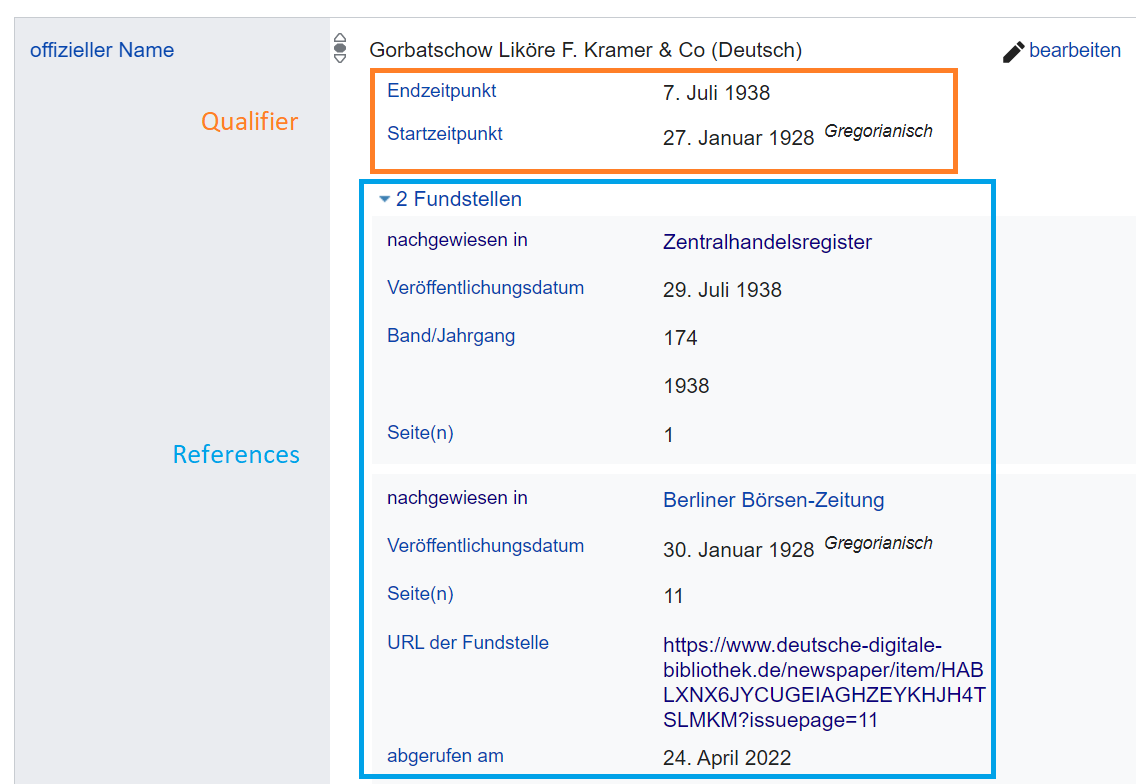
\includegraphics[width=\ScaleIfNeeded]{wikidata-reference}}
    \caption{Qualifikator und Fundstellen zu der Namensform ,,Gorbatschow Liköre F. Kramer \& Co'' des gleichnamigen Gewerbebetriebs.}
    \label{fig:x cubed graph}
\end{figure}

Wie in der Abbildung 4.9 an der zweiten Fundstelle außerdem zu sehen ist, kann ein permanenter Link zum gegenbenfalls im Web vorhandenen Quellendigitalisit hinterlegt werden. Falls dieses in einer Open Data-Lizenz veröffentlicht ist, bietet sich darüber hinaus an, es direkt in das Schwesternprojekt und in die öffentliche Bildersammlung \textit{Wikimedia Commons}\footnote{URL: \url{https://commons.wikimedia.org/wiki/Hauptseite} (letzter Zugriff am 28.05.2022).} hochzuladen. Dort gibt es bereits Bildmaterial zu Jüdischen Gewerbebetrieben vor allem in Zusammenhang mit der Reichspogromnacht 1938 sowie mit announcierten Besitzübernahmen, das bei zugehörigen Wikidata-Items direkt eingebunden werden kann (Abbildung 4.10).\footnote{Siehe Abfrage zu ,,Arisierung'' in Commons, URL: \url{https://commons.wikimedia.org/w/index.php?search=Arisierung&title=Special:MediaSearch&go=Go&type=image} (letzter Zugriff am 28.05.2022).}

\begin{figure}[h]
    \centering
    \frame{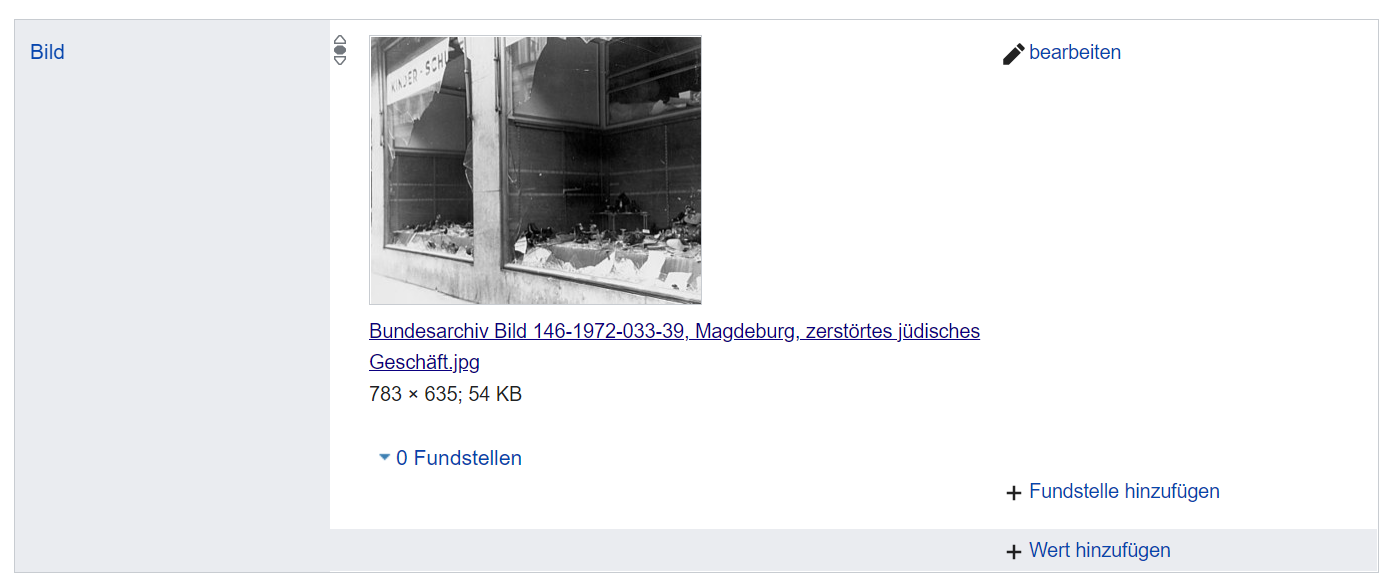
\includegraphics[width=\ScaleIfNeeded]{wikidata-commons}}
    \caption{Direkte Verknüpfung eines Fotodigitalisats aus Wikimedia Commons in Wikidata.}
    \label{fig:x cubed graph}
\end{figure}

Daraus ergibt sich erstmalig eine direkte Verknüpfung von Forschungsdaten und historischen Quellen, die eine bisher nie dagewesene Datenüberprüfung und -verifizierung ermöglicht und in der Konsequenz die Glaubwürdigkeit von Forschungsdaten im Forschungsfeld enorm steigern kann.\footnote{Auch in den Interviews wurde eine mögliche Verknüpfung als Funktionalität von offenem Forschungsdatenmanagement herausgehoben, vgl. Interview B3\_Transkript, Pos. 77.} 

Das Wikidata-Projekt kann daneben zur methodischen Führung sowie zur Entwicklung von Kriterien, welche Quellen sich als Belege für Jüdische Gewerbebetriebe eignen, genutzt und eine qualifzierte Quellensammlung im Forschungsfeld sukzessive aufgebaut werden.

\subsection{Erfassung von jüdischen Gewerbebtrieben}

Für die Erfassung der Daten zu jüdischen Gewerbebetriebe, so geht es aus den Interviews hervor, kamen herkömmliche Microsoft-Produkte wie Excel oder Access zum Einsatz.\footnote{Vgl. Interview B3\_Transkript, Pos. 11 und Interview B2\_Transkript, Pos. 27.} Es wurde folglich in erster Linie proprietäre, also kostenpflichtige, Software genutzt, die in der Regel nicht plattformunabhängig ist. Dies erschwert generell eine kollaborative Arbeit auf den Daten, denn die MS-Access-Anwendung zum Beispiel steht für Unix-basierte Betriebssysteme (Linux, Apple) gar nicht oder nur eingeschränkt zur Verfügung. Das heißt, dass grundlegende Open Source-Kritierien von diesen Produkten nicht erfüllt werden. 

Im Zusammenhang mit der Datenerfassung ist daher die wohl größte Herausforderung und aufwändigste Arbeit, ein User-Interface (UI) zu gestalten, das die bestmögliche User Experience und Usability (UX) bietet. Hier hält Wikidata nicht die perfekte Lösung bereit, aber zumindest Auswege aus möglichen anwendungsbedingten Einschränkungen und Zwängen, indem es nicht nur eine sondern mehrere Möglichkeiten der Erfassung von Daten gibt.\footnote{Siehe Wikidata:Datenspende, URL: \url{https://www.wikidata.org/wiki/Wikidata:Data\_donation/de\#Online-Tools\_=} (letzter Zugriff am 29.05.2022).} Von diesen werden drei nachfolgend vorgestellt, die sich an den bisherigen Kenntnisständen und Erfahrungen mit digitalen Werkzeugen im Forschungsfeld orientieren. 

Naheliegend ist die Eingabe der Daten im Linked Open Data Interface direkt auf der Website von Wikidata, wo per Mouseclick eines neues einzelnes Datenobjekt erstellt und erfasst werden kann (Abbildung 4.11). 

\begin{figure}[h]
    \centering
    \frame{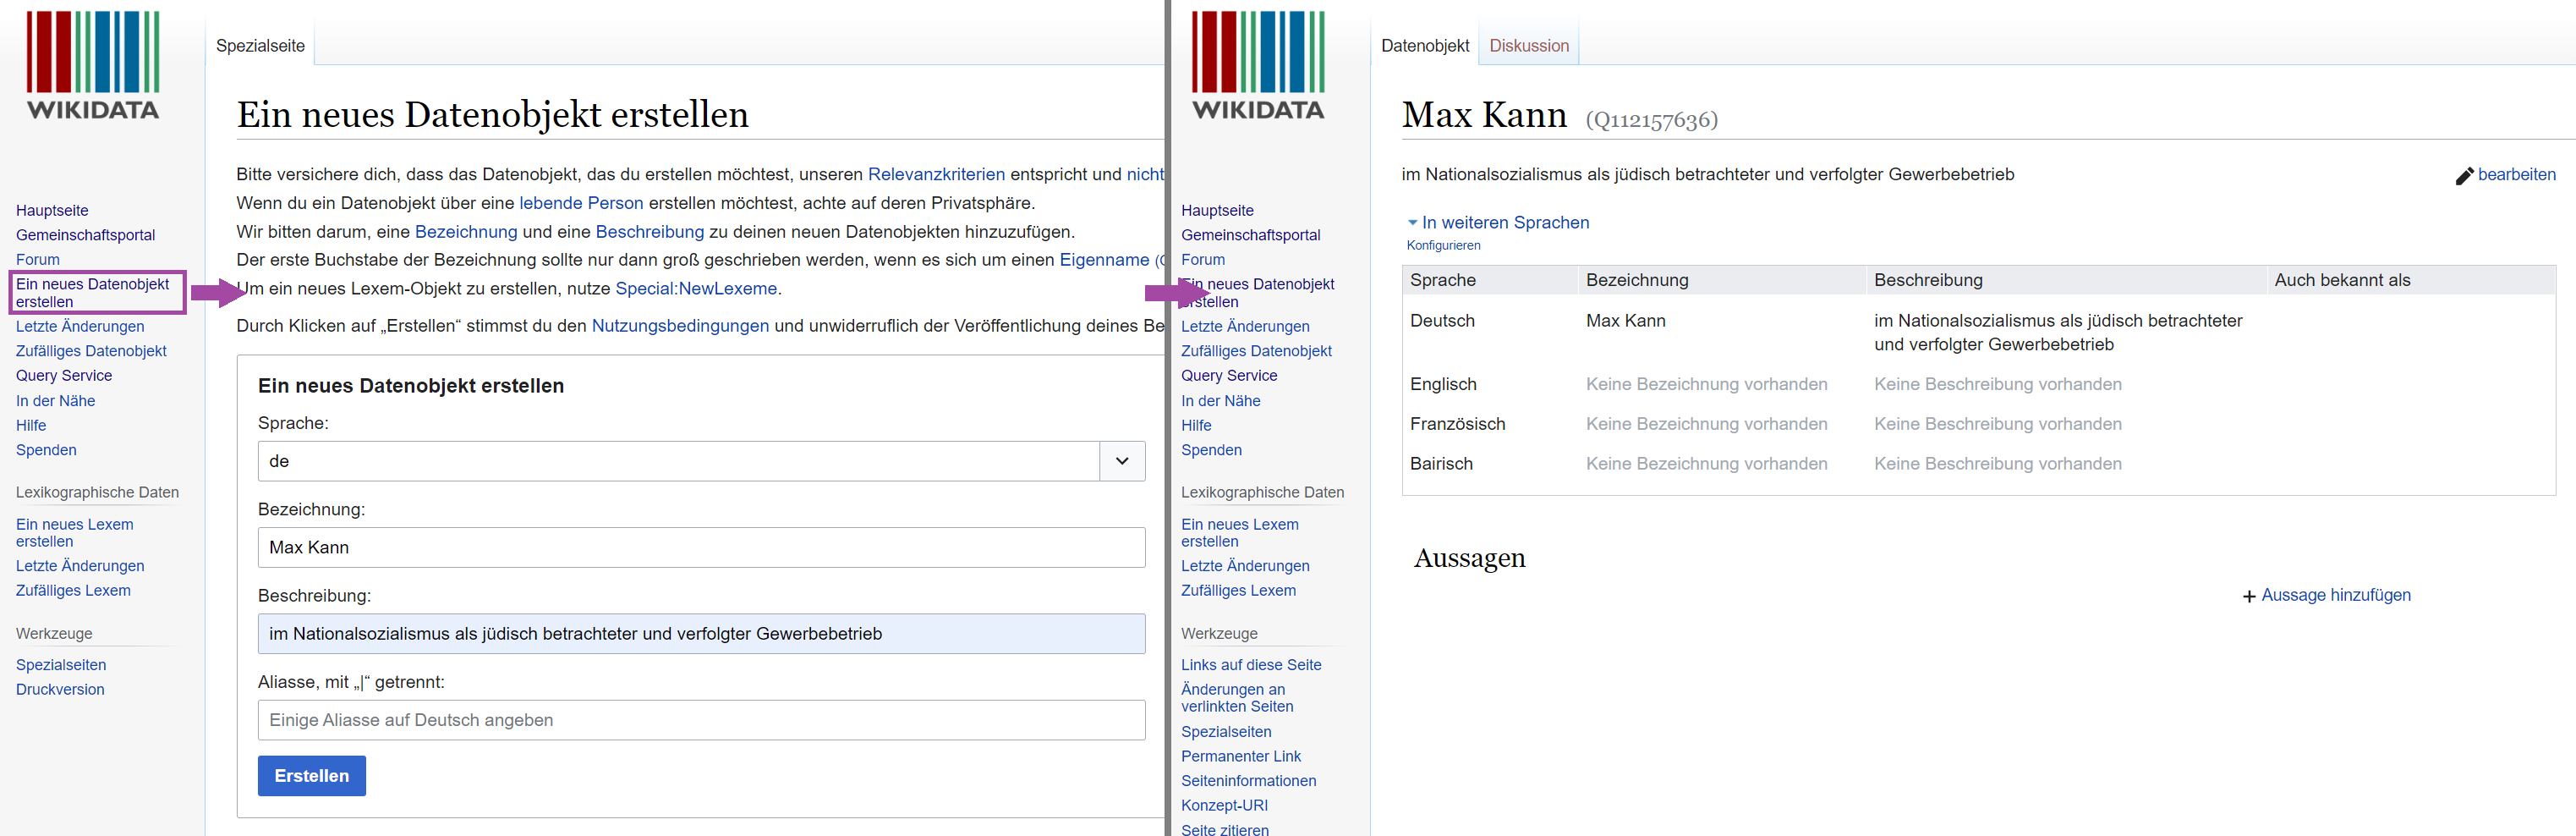
\includegraphics[width=\ScaleIfNeeded]{wikidata-linked-data-interface}}
    \caption{Links im Bild wird das Datenobjekt ,,Max Kann'' angelegt. Rechts ist das Item erstellt worden und es können weitere Daten erfasst werden.}
    \label{fig:x cubed graph}
\end{figure}

Diese Möglichkeit eignet sich besonders gut, wenn nur wenige Jüdische Gewerbebetriebe zur erfassen sind. Der Vorteil ist auch, dass ein Team gleichzeitig an der Eingabe von Daten arbeiten kann, was in den älteren Excel- oder Access-Desktopversionen nicht nicht möglich war.\footnote{Seit den Webversionen der Office-Sammlung von Microsoft kann allerdings auch in diesen kollaborativ gearbeitet werden. Siehe Microsoft Support (2022): Gleichzeitiges Bearbeiten von Excel-Arbeitsmappen mit der gemeinsamen Dokumenterstellung, URL: \url{https://support.microsoft.com/de-de/office/gleichzeitiges-bearbeiten-von-excel-arbeitsmappen-mit-der-gemeinsamen-dokumenterstellung-7152aa8b-b791-414c-a3bb-3024e46fb104}.} Mit steigender Zahl kann die Eingabe im Wikidata-Interface jedoch an Grenzen stoßen. Für Berlin, Frankfurt a.M. sowie Mannheim wurden jeweils Daten im 1.000er-Bereich erhoben.\footnote{In Berlin ca. 8.000, Frankfurt a.M. ca. 3.000 und Mannheim ca. 1.200.} Diese alle manuell und einzeln einzugeben, kostet vor allem Zeit, zumal diese bereits in Tabellenform vorliegen. In diesem Fall bietet sich die Stapel-Importfunktion (batch import) ,,QuickStatements'' an, bei der Daten, die als Tabstopp- oder Komma-separierte strukturierte Daten vorliegen, in Wikidata importiert werden.\footnote{URL: \url{https://quickstatements.toolforge.org/\#/batch} (letzer Zugriff am 29.05.2022).} Bevor der eigentliche Import jedoch erfolgen kann, bedarf es der Vorbereitung und Bereinigung der Daten. Zuerst müssen proprietären Formate in das offene CSV-Format transformiert werden, was zumindest für Excel-Dateien unproblematisch mit der Exportfunktion erfolgen kann (Abbildung 4.12).

\begin{figure}[h]
    \centering
    \frame{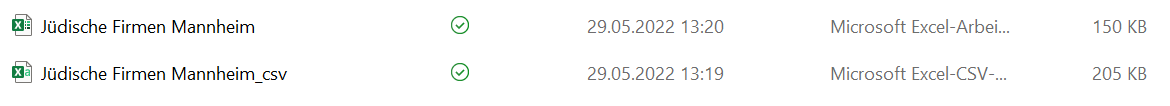
\includegraphics[width=\ScaleIfNeeded]{excel-csv}}
    \caption{Export der Excel-Tabelle mit Daten zu Jüdischen Gewerbebetrieben aus Mannheim in das CSV-Format.}
    \label{fig:x cubed graph}
\end{figure}

Bei den Access-Datenbanken ist diese Transformation aufwändiger, da hier das Problem hinzu kommt, dass es sich um veraltete Software-Versionen (2007) handelt, die sich mit neueren Versionen nicht mehr so einfach öffnen lassen. Für Berlin wurde kürzlich in einem eigenen Projekt diese Transformation durchgeführt.\footnote{Siehe Kapitel 1 Einleitung.} Im nächsten Schritt muss die ursprüngliche Datenstrukturierung in den transformierten CSV-Dateien an das Datenmodell des Wikidata-Projekts angepasst werden, wofür Wikidata ausführliche Hilfestellungen bereitgestellt hat.\footnote{Siehe Wikidata Help:QuickStatements, URL: \url{https://www.wikidata.org/wiki/Help:QuickStatements} (letzter Zugriff am 29.05.2022).} Dies wurde am Beispiel des Gewerbebetriebs \textit{Franz Mettner GmbH} aus Mannheim\footnote{URL (stable): url{https://www.wikidata.org/w/index.php?title=Q112163392\&oldid=1649916700}.} getestet (Abbildung 4.13).

\begin{figure}[h]
    \centering
    \frame{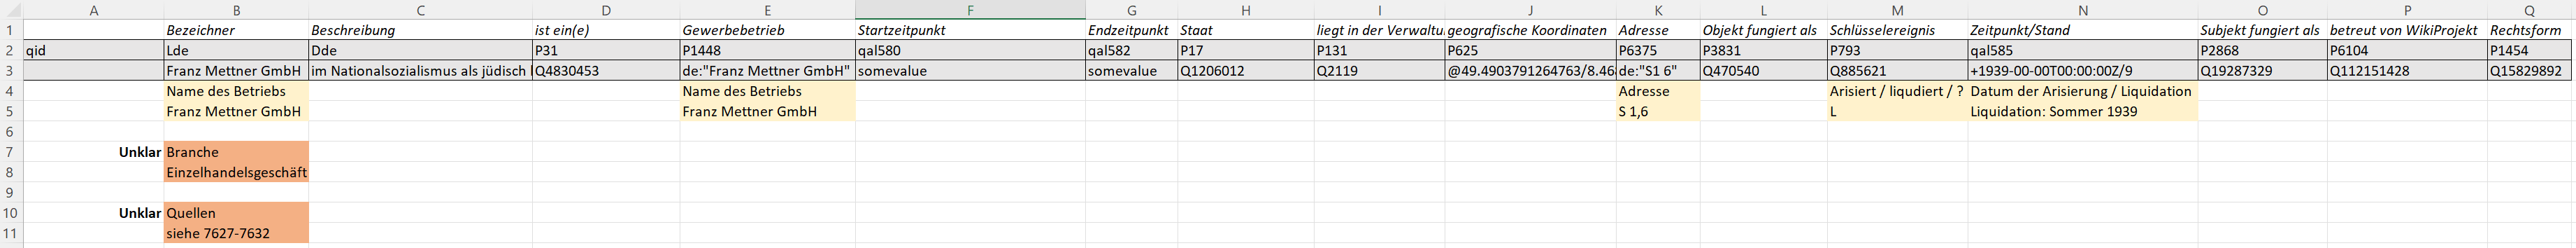
\includegraphics[width=\ScaleIfNeeded]{wikidata-bereinigung}}
    \caption{Datenvorbereitung und -bereinigung für den Import mit ,,QuickStatements''.}
    \label{fig:x cubed graph}
\end{figure}

Grau hinterlegt sind die Komma-separierten Werte, welche mit QuickStatements importiert wurden. Gelb und orange markiert sind die ursprünglichen Felder aus der Excel-Tabelle, welche dem Wikidata-Datenmodell zugeordnet werden konnten (gelb) und die Schwierigkeiten bereitet haben (orange). So scheint die Einordnung von ,,Einzelhandelsgeschäft'' unter Branche nicht treffend zu sein. Zudem sind die Quellenangaben ,,siehe 7627-7632'' nicht überprüfbar. Eventuell beziehen sich die Nummern auf ein projektinterne Verzeichnis, das aber nicht verfügbar ist. Das bedeutet, dass eine Verifizierung des Jüdischen Gewerbebetriebs allein mit der Excel-Tabelle für Externe nicht möglich ist. Hier müsste demnach vor dem Import die exakten Quellenangaben noch ergänzt werden. Der Import selbst in QuickStatements ist, sofern das Schema in der CSV-Datei korrekt ist, schnell erledigt (Abbildung 4.14).

\begin{figure}[h]
    \centering
    \frame{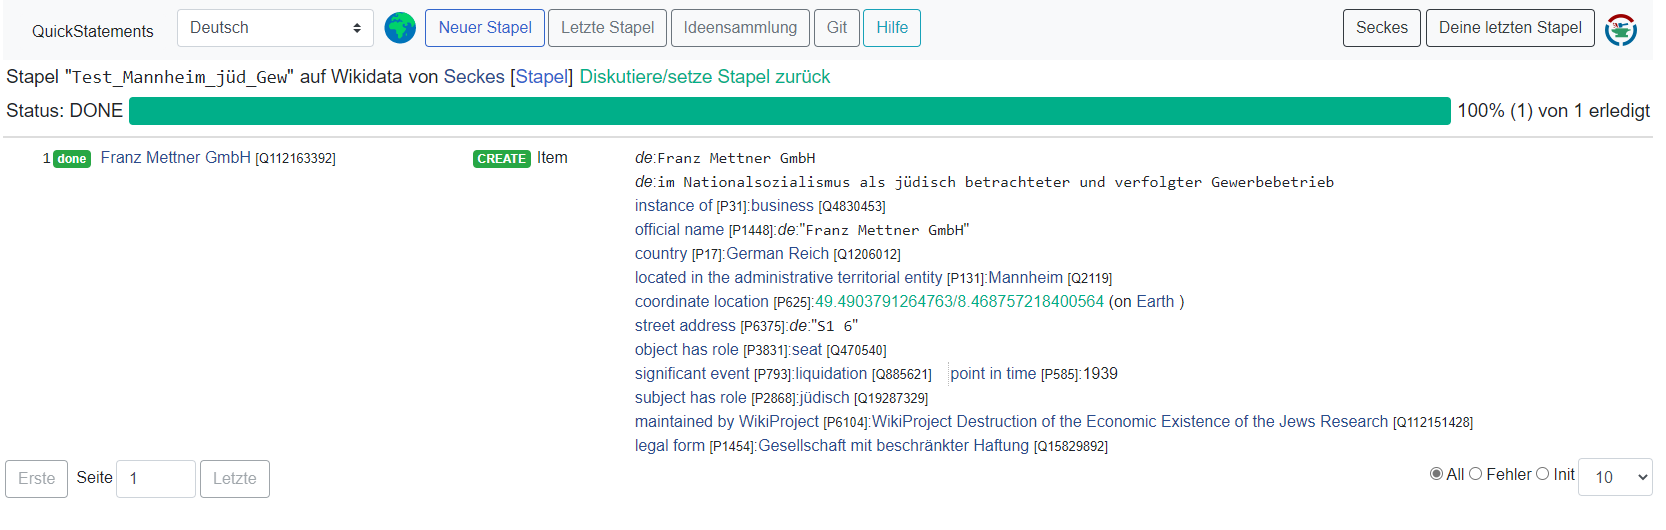
\includegraphics[width=\ScaleIfNeeded]{wikidata-quickstatements}}
    \caption{Erfolgreicher Import in QuickStatements.}
    \label{fig:x cubed graph}
\end{figure}

Während des Test-Imports zeigte sich, dass vor allem die Vorbereitung und Bereinigung der Daten für den Import zeitintensiv ist. Hier tauchen schließlich auch Probleme auf, die nicht immer vorhersehbar sind und für die eine Lösung gefunden werden muss. Dies betrifft insbesondere auch Freitextfelder, die von allen Studien verwendet und in denen unterschiedlichste Informationen festgehalten wurden. Diese lassen sich in Wikidata nicht importieren. Es ist nicht klar, welche Rolle diese Felder später bei der Auswertung spielten. Statistisch lässt sich damit jedenfalls nicht arbeiten. In einigen Fällen lassen sich die enthaltenen Daten auf den ersten Blick normalisieren, wenn zum Beispiel ,,1937 Emigration in die USA'' vermerkt ist. Schwieriger wird es bei Anmerkungen wie ,,1910 verlegte er sein Geschäft nach Mannheim (4-5 Arbeiter, die Ehefrau und der Sohn haben auch dort gearbeitet); 1937: wegen Hehlerei zu 1 Jahr, 4 Monaten und 2 Wochen Haft verurteilt Verbot zur Weiterführung des Geschäfts für 3 Jahre; nach USA emigiert''. Hieraus lassen sich drei Informationen extrahieren, die empirisch interessant sein können: Umzug, Anzahl Angestellte, Schicksal des Eigentümers. Wichtig wäre hier auch die Entscheidung, welche Daten nicht gebraucht und folglich kassiert werden.

\begin{figure}[h]
    \centering
    \frame{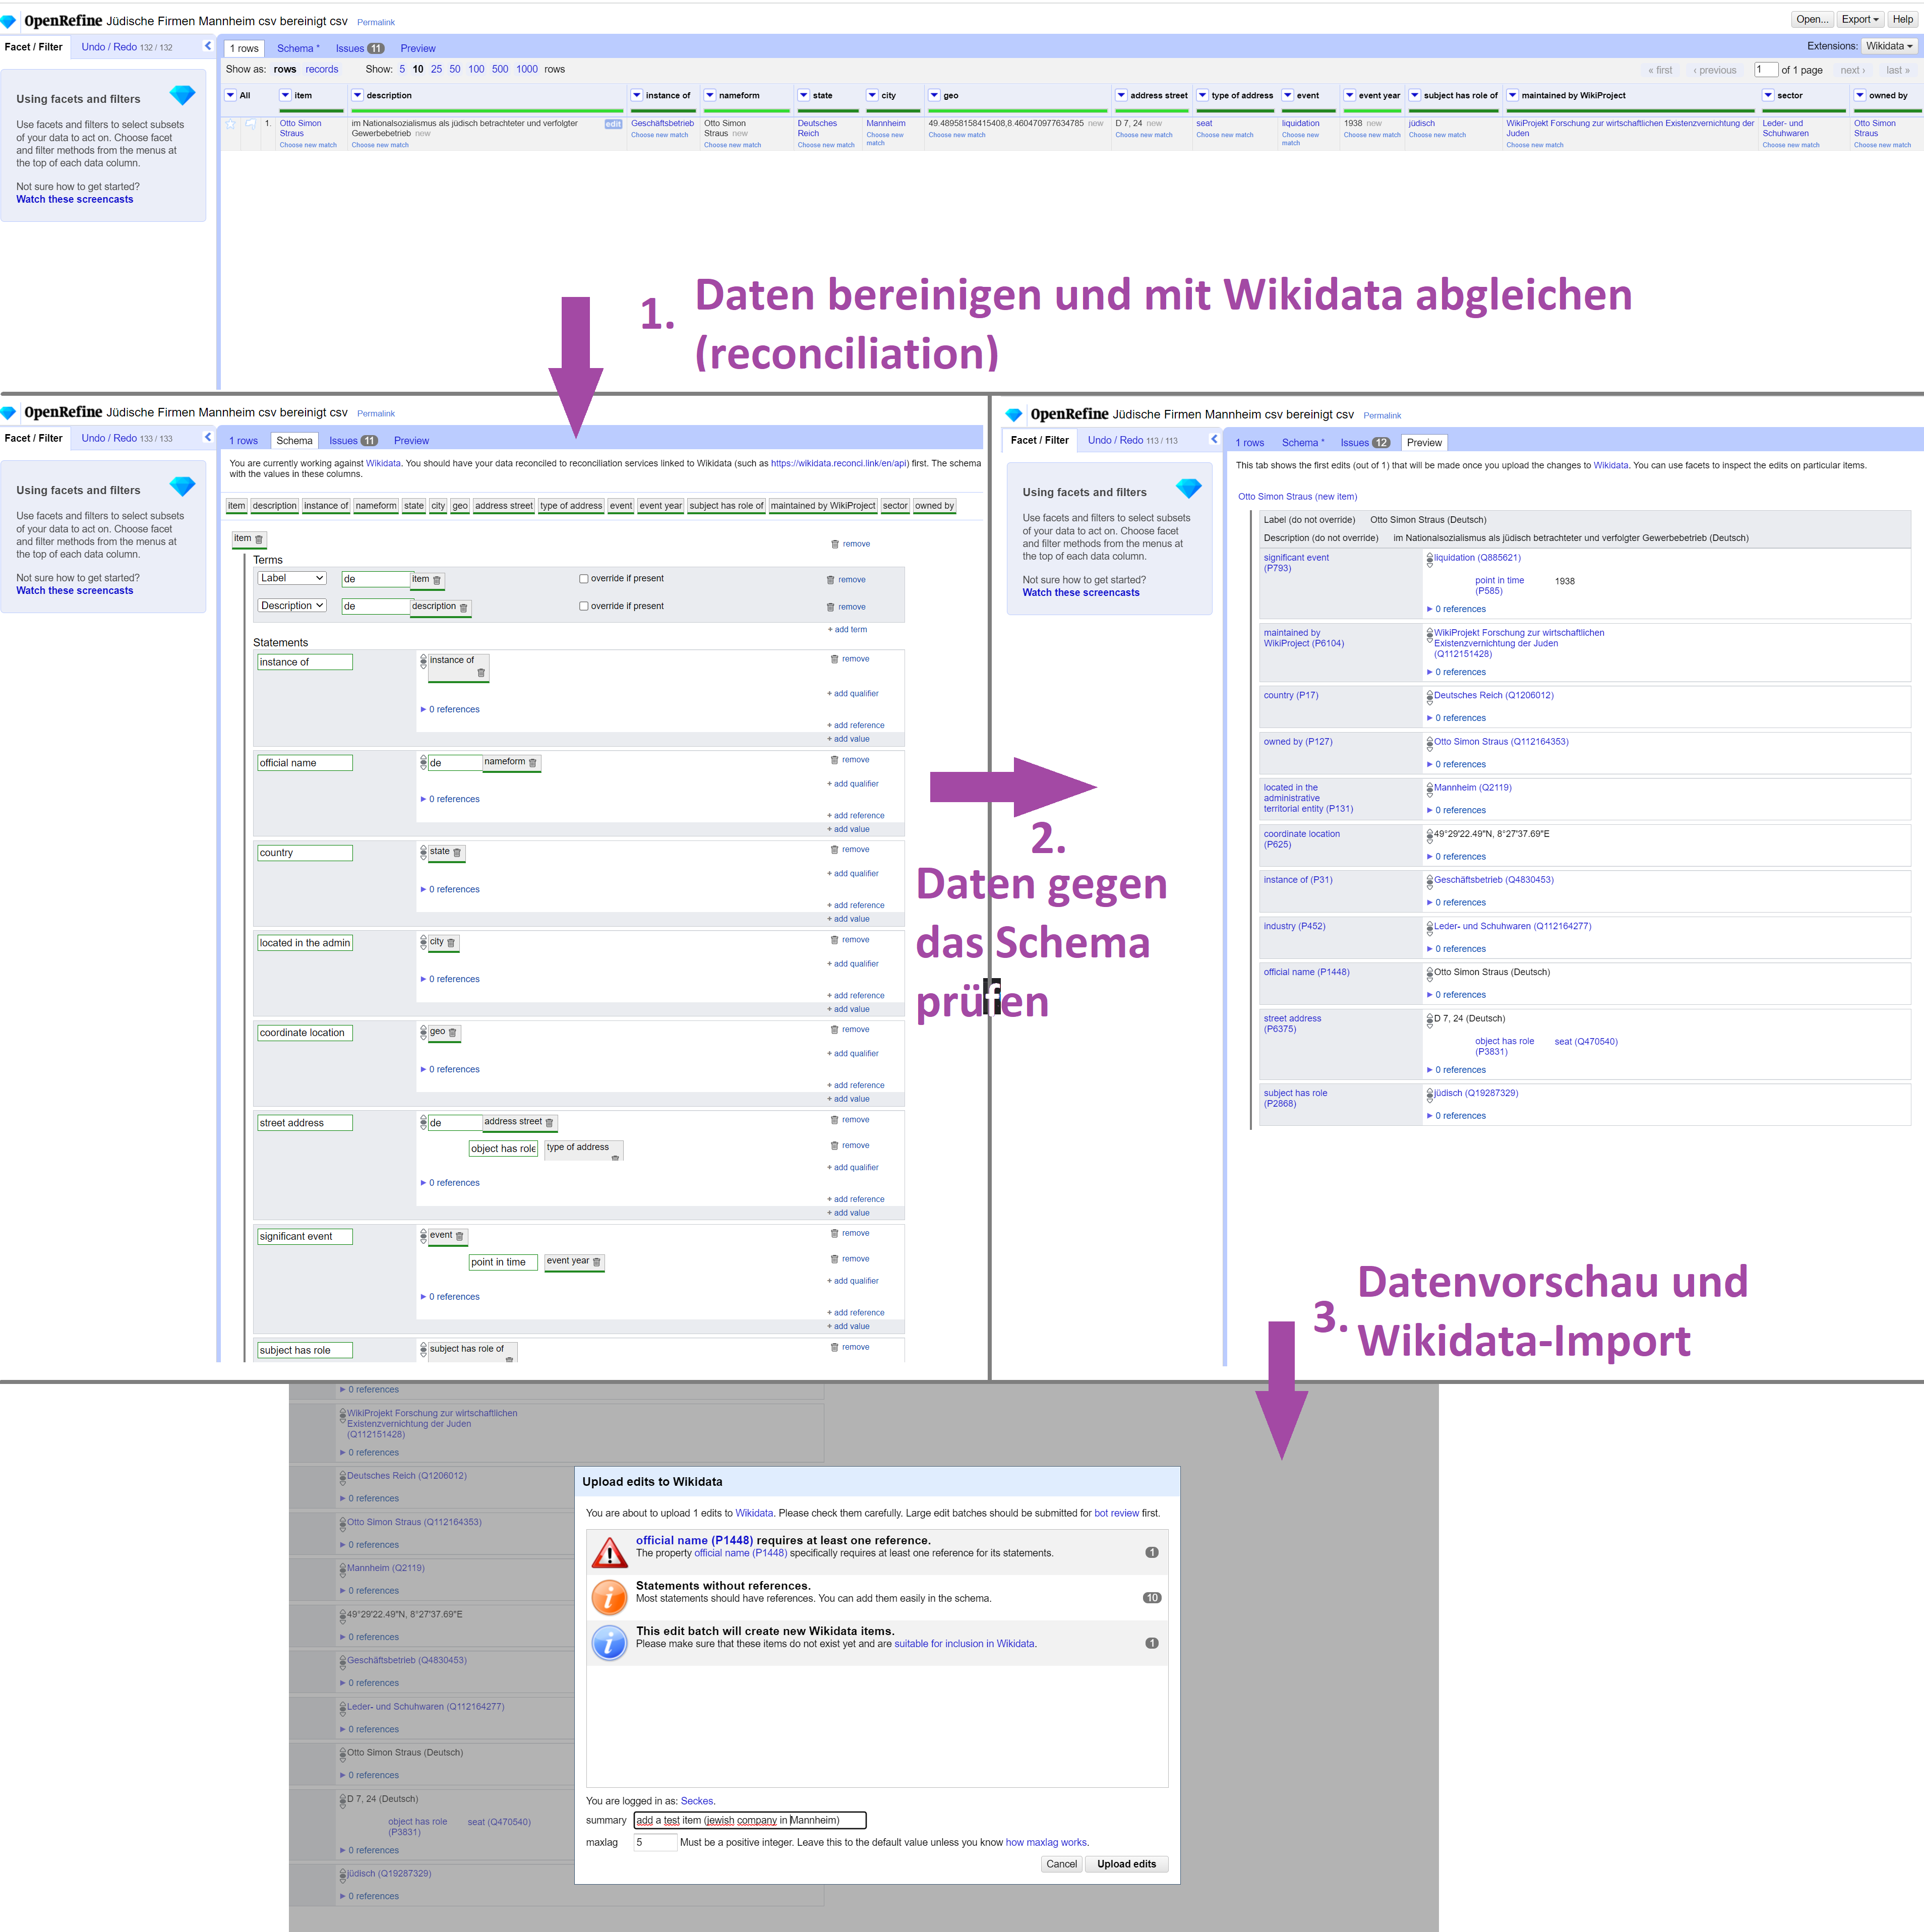
\includegraphics[width=\ScaleIfNeeded]{wikidata-pipeline}}
    \caption{Wikidata-Pipeline in Open Refine.}
    \label{fig:x cubed graph}
\end{figure}

Die dritte und letzte Option, die in dieser Arbeit vorgestellt wird, verdeutlicht, wie mit Wikidata Pipelines genutzt werden können, um optimale Workflows für die Datenerfassung in die Forschungsarbeit zu integrieren. Denn ein Nachteil von QuickStatements ist, dass die Daten aus den CSV-Dateien manuell in die Webanwendung kopiert werden müssen. Außerdem können die Daten in der Anwendung selbst nicht weiter überprüft werden. Hierfür ist das Open Source-Tool ,,Open Refine''\footnote{URL: \url{https://openrefine.org/} (letzter Zugriff am 29.05.2022).} besser geeignet. Die mächtige Anwendung, die auf die Bereinigung und Anreicherung von Massendaten spezialisiert ist, ermöglicht den Abgleich der Tabellendaten mit externen Wissensdatenbanken und darüber hinaus den Import direkt aus der Anwendung nach Wikidata (Abbildung 4.15).\footnote{Siehe Wikidata:Tools/OpenRefine, URL (stable:) \url{https://www.wikidata.org/w/index.php?title=Wikidata:Tools/OpenRefine\&oldid=1620901604}, Open Refine (2022): Overview of Wikibase support. Editing Wikidata with OpenRefine, URL: \url{https://docs.openrefine.org/manual/wikibase/overview\#editing-wikidata-with-openrefine} (letzter Zugriff am 29.05.2022).}

Die Kernfunktionen der Datenbereinigung werden hier nicht weiter erläutert, sondern auf die Wikidata-Upload-Pipeline fokussiert. In Abbildung 4.15 sind die Daten zum Jüdischen Gewerbebetrieb \textit{Otto Simon Straus} aus Manneheim\footnote{URL (stable): \url{https://www.wikidata.org/w/index.php?title=Q112166241\&oldid=1650023676}.} bereits von einer CSV-Datei in neu erstelltes Open Refine-Projekt hochgeladen worden. Die farbigen Balken unter jeder Titelspalte zeigen den Status des Abgleichs der Daten mit Wikidata an, welcher in Open Refine als ,,Reconciliation process'' bezeichnet wird. Dieser muss einmal für jede Titelspalte vorgenommen. Die dunkelgrünen Balken stehen für eindeutige Treffer (Abbildung 4.16 am Beispiel ,,Liquidation''), die hellgrünen für neue Werte und die grauen Balken für die noch abzugleichenden Daten. 

\begin{figure}[h]
    \centering
    \frame{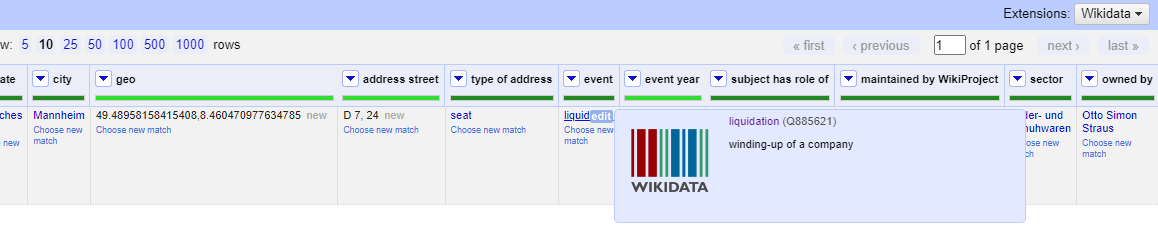
\includegraphics[width=\ScaleIfNeeded]{wikidata-reconciliation}}
    \caption{Eindeutiger Abgleich mit Wikidata in Open Refine.}
    \label{fig:x cubed graph}
\end{figure}

Im zweiten Schritt (in der Abbildung in der Mitte links) erfolgt die Prüfung der abgeglichenen Daten gegen ein Wikidata-Schema. Dies kann entweder direkt in Open Refine erstellt oder ein bestehendes als JSON-File importiert werden. Wenn für die Jüdischen Gewerbebetriebe demnach ein grundlegendes Datenmodell feststeht, kann dieses als JSON zum Beispiel im Wikidata-Projekt zur Verfügung gestellt und von jedem/ jeder in Open Refine wiederverwendet werden.\footnote{Zum Test wurde das in Open Refine erstellte Schema im Wikidata-Projekt hochgeladen, siehe URL: \url{https://www.wikidata.org/wiki/Wikidata:WikiProject\_Destruction\_of\_the\_Economic\_Existence\_of\_the\_Jews\_Research/Vernichtung\_der\_jüdischen\_Gewerbetätigkeit/Schema}.} Auf diese Weise sich eine Datenkontrolle bei der Dateneingabe im Forschungsfeld forcieren, was insgesamt zur Datenqualität beiträgt. Zum anderen ist es eine Arbeitserleichterung und bietet methodische Führung, wenn Schemata nachgenutzt und nicht für jedes Projekt von Grund auf neu erstellt werden müssen. Im dritten und letzten Schritt der Pipeline (Abbildung in der Mitte rechts sowie unten) lassen sich die Daten in einer Vorschau in Open Refine nochmals überprüfen, bevor sie in Wikidata importiert werden.\footnote{Permalink zum lokalen Projekt (localhost) URL: \url{http://127.0.0.1:3333/project?project=2437124036317\&ui=\%7B\%22facets\%22\%3A\%5B\%5D\%7D}.} Der Nachteil von Open Refine ist, dass die Möglichkeiten der kollaborativen Arbeit an einem Projekt noch begrenzt sind. Bisher können diese nur manuell zusammengeführt werden.\footnote{Siehe Consortium Historicum (2018): Ergänzen eines OpenRefine-Projekts mit einem anderen, Blogbeitrag auf histHub am 26.02.2018, URL: \url{https://histhub.ch/ergaenzen-eines-openrefine-projekts-mit-einem-anderen/} (letzter Zugriff am 30.05.2022).} 

Auch wenn die diversen Möglichkeiten des Datenimports in Wikidata zunächst überfordern können\footnote{Neben den drei vorgestellten Tools gibt es auch noch die REST-Api von Wikimedia sowie die Möglichkeit der Verwendung von Bots. Auch Wikimedia Cloud Services-Projekte mit weiteren Werkzeugen befinden im Aufbau, URL: \url{https://wikitech.wikimedia.org/wiki/Help:Cloud_Services_introduction} (letzter Zugriff am 30.05.2022).}, ist der Vorteil insgesamt, dass durch diese Vielseitigkeit die Datenerfassung an jeweilige Use Cases und an Nutzungsgewohnheiten optimal angepasst werden kann. Auch vor dem Hintergrund, dass immer mehr historische Quellen digitalisiert vorliegen, was einen automatisierten Import ermöglicht, werden diese vielfältigen Services des Datenimports zunehmend notwendig.\footnote{Das NFDI-Konsortium nfdi4Culture organisiert Ende Juni einen Workshop, der sich explizit mit der Wikibase-Upload-Pipeline in Open Refine beschäftigt, siehe URL: \url{https://nfdi4culture.de/news-events/events/jcdl-workshop-open-refine-to-wikibase-a-new-data-upload-pipeline.html} (letzter Zugriff am 29.05.2022).} Die Kehrseite dieser Werkzeugvielfalt ist, dass sich die Einarbeitungszeit mit jedem neuen Tool, das genutzt wird, insgesamt verlängert.

\subsection{Verknüpfung von Sample und Fallbeispielen}

Mehrmals wurde in den Interviews betont, dass die rein quantitative Arbeit im Forschungsfeld lediglich einen Teil der Forschung zur Vernichtung der jüdischen Gewerbetätigkeit ausmacht.\footnote{Vgl. Interviews B2\_Transkript, Pos. 53, 63 und B3\_Transkript, Pos. 83.} Den anderen Teil bilden Fallbeispiele, die vor allem zeigen, dass der Prozess der Verfolgung und Vernichtung von zahlreichen Einzelfaktoren abhing und auf der individuellen Ebene daher sehr unterschiedlich verlaufen konnte. Neben diesen Einzelfallstudien gibt es außerdem die Gedenkbücher in analoger oder digitaler Form, die einen stark dokumentarischen Charakter aufweisen, der sich vorwiegend in einem deskriptiven Zusammentragen von verteilten Informationen zu jüdischen Gewerbebetrieben und jüdischen Unternehmern zeigt.\footnote{Nietzel hebt hier die akribisch recherchierte Textsammlung zu jüdischen Unternehmen in München des Archivars und Historikers Wolfgang Selig aus dem Jahr 2004 hervor, vgl. Nietzel 2009, S. 583.} Hierunter zählen auch jene Veröffentlichungen, die nicht primär auf Daten zu jüdischen Gewerbebetrieben fokussiert sind, sondern wo diese von anreichernder Bedeutung sind.\footnote{Hier vor allem die zahlreichen Gedenkbücher zu jüdischen Personen, die mittlerweile online zugänglich sind und wo sich Daten zu jüdischen Gewerbebetrieben in den Biogrammen der Personen ,,verstecken''. Siehe zum Beispiel ,,Biografisches Gedenkbuch der Münchner Juden 1933–1945'' der Stadt München, URL: \url{https://gedenkbuch.muenchen.de/} (letzter Zugriff am 12.05.2022). Bei der Biografie von Max Hofman ist unter ,,Weitere Informationen'' vermerkt: ,,Max Hofmann war Inhaber der Fa. Max Hofmann, einem Großhandel und Versand von Manufaktur- und Textilwaren, in der Paul-Heyse-Straße 28/I. Das Gewerbe wurde am 17.10.1938 für den 15.10.1938 abgemeldet.'', URL (stable): \url{https://gedenkbuch.muenchen.de/index.php?id=gedenkbuch_link&gid=5722}.} Diese Datenvielfalt im Forschungsfeld lässt sich wie folgt zusammenfassen: 

\begin{enumerate}
    \item Es gibt \textbf{quantitative (Massen-)Daten}, die strukturiert, entweder als Rohdaten oder in aggregierter Form, vorliegen. Sie besitzen eine statistische Aussagekraft.
    \item Es gibt \textbf{qualitative Daten}, die in der Regel textuell und damit unstrukturiert oder semistruktiert vorliegen.
\end{enumerate}

Bereits Nietzel beklagte in seinem Forschungsbericht aus dem Jahr 2009, dass die qualitativen Daten insbesondere aus der Gedenk- und Erinnerungskultur für eine wissenschaftliche analytische Auswertung bislang zu unsystematisch sind.\footnote{Nietzel 2009, S. 583.} Umgekehrt fehlt den statistischen Massendaten ihres Umfang wegens oft die entsprechende Datentiefe und die Einzelschicksale und -geschichten hinter der Statistik bleiben unsichtbar.\footnote{Allein für Berlin hat die Stichprobe einen Umfang von ca. 8.000 jüdischen Gewerbebetrieben. Auch für Frankfurt am Main sind es in der Stichprobe über 2.500 jüdische Gewerbebtriebe. Vgl. Kreutzmüller 2012, URL: \url{https://www2.hu-berlin.de/djgb/www/find} (letzter Zugriff am 07.05.2022) und Nietzel 2012, S. 15.} Das macht diese Daten vor allem außerhalb der wissenschaftlichen Forschung weniger greif- und nutzbar. 

\begin{figure}[h]
    \centering
    \frame{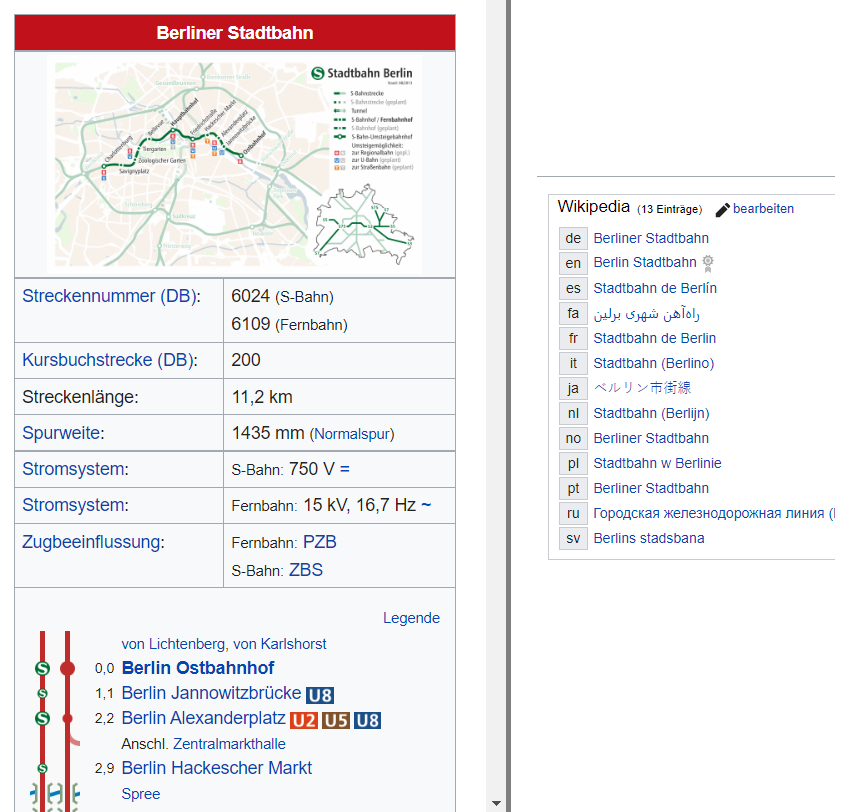
\includegraphics[scale=0.4]{wikidata-wikipedia}}
    \caption{In Wikipedia werden Wikidata-Daten üblicherweise für kompakte Infoboxen genutzt, hier am Beispiel des Artikels zur Berliner Stadtbahn (links). In Wikidata wiederum lässt sich dem Item Berliner Stadtbahn (Q694223) der Wikipedia-Artikel aller Sprachversionen eindeutig zuordnen (rechts).}
    \label{fig:x cubed graph}
\end{figure}

Festzuhalten ist, dass es bisher im Forschungsfeld noch nicht gelungen ist, quantitative und qualitative Forschungsdaten zu verknüpfen. Es ist aber eben diese Verknüpfung der verteilten Datenvielfalt, die im Wiki*versum gängige Praxis ist. Dies wurde bereits anhand der Quellendigitalisite in ,,Wikimedia Commons'' und deren Integration in Wikidata deutlich.\footnote{Vgl. Kapitel 4.3.2 Quellennachweise.} Gleiches lässt sich auch auf der Textebene mit der Enzyklopädie \textit{Wikipedia} realisieren. Analog zu Wikidata-Projekten gibt es in der Wikipedia Themenportale, die sich auf das Schreiben von Wikipedia-Artikeln zu einem bestimmten Thema spezialisiert haben.\footnote{Portal:Wikipedia nach Themen, URL: \url{https://de.wikipedia.org/wiki/Portal:Wikipedia_nach_Themen} (letzter Zugriff am 30.05.2022).} Unter den Rubriken ,,Geschichte'' oder ,,Wissenschaft'' gibt es thematisch dem Forschungsfeld nahestehende Portale wie das ,,Portal:Geschichte des 20. Jahrhunderts''\footnote{URL (stable): \url{https://de.wikipedia.org/w/index.php?title=Portal:Geschichte\_des\_20.\_Jahrhunderts\&oldid=216577544}.} oder ,,Portal:Geschichte''\footnote{URL (stable): \url{https://de.wikipedia.org/w/index.php?title=Portal:Geschichte\&oldid=215435556}.} Es kann jedoch auch ein neues Themenportal angelegt werden. Im Wikipedia-Artikel können die strukturierten Daten aus Wikidata üblicherweise in einer kompakten Infobox hinzugefügt werden, während dem zugörigen Wikidata-Item der Wikipedia-Artikel verknüpft wird (Abbildung 4.16).\footnote{Siehe zur Umsetzung der Verknüpfungen die Dokumentationsseite ,,Wikidata:Wie man Daten in Wikimedia-Projekten nutzt'', URL: \url{https://www.wikidata.org/wiki/Wikidata:How_to_use_data_on_Wikimedia_projects/de} (letzter Zugriff am 30.05.2022).}

Im Rahmen dieser Arbeit liegt der Schwerpunkt auf den strukturierten (Massen)Daten und damit auf Wikidata. Somit bleiben die Möglichkeiten der Verbindung zu Wikipedia hier nur angedeutet. Sie zeigen aber bereits die Potentiale, die sich über Wikidata hinaus im Wiki*versum für das Forschungsfeld ergeben. So können kollaborativ ,,Geschichten'' zu Jüdischen Gewerbebetrieben gesammelt und diese in Wikipedia-Artikeln veröffentlicht werden, die für alle zugänglich und nachnutzbar sind. Gleichzeitig können aus den Artikeln Daten extrahiert, strukturiert in Wikidata erfasst und dort ebenfalls nachgenutzt werden.

\section{Analyse}

Für die finale Datenauswertung kam im Forschungsfeld einfache deskriptive Statistik zur Anwendung. Es ging also zuvorderst darum, die Forschungsdaten zu Jüdischen Gewerbebetrieben den Forschungsfragen entsprechend zu ordnen und übersichtlich darzustellen. Dies geschah überwiegend in Tabellenform. Nur im Fall von Berlin wurden die Daten auch mit Karten, Balken- und Liniendiagrammen visualisiert. In dieser aggegrierten Form sind sie in den Publikationen der Lokalstudien zugänglich. Mit welchen Tools exakt die Datenauswertung der einzelnen Studien erfolgte, ist nicht bekannt. Aus den Lokalstudien lässt sich aber schließen, dass für die Datenanalyse in der Regel einfache Datenabfragen (Queries) ausreichen. 

Wikidata bietet neben der Speicherung von Daten auch deren Abfrage mit dem ,,Wikidata Query Service'' an.\footnote{Wikidata Query Service, URL: \url{https://query.wikidata.org/} (letzter Zugriff am 30.05.2022).} Dies erfolgt in der globalen Linked Open Data- und RDF-Abfragesprache \textit{SPARQL} (SPARQL Protocol And RDF Query Language), welche seit 2013 vom ,,World Wide Web Consortium'' (W3C) als offizielle Spezifikation veröffentlicht und folglich zum Standard erklärt wurde.\footnote{Vgl. W3C (2013): SPARQL 1.1 Overview. W3C Recommendation 21 March 2013, URL: \url{http://www.w3.org/TR/2013/REC-sparql11-overview-20130321/} (letzter Zugriff am 30.05.2022).} Ein grundlegender Unterschied zur konventionellen SQL-Datenabfragesprache (Structured Query Language) in relationalen Datenbanken besteht darin, dass mit SPARQL unter der Verwendung von ,,Namespaces'' über Datenquellen hinweg Daten abgefragt werden können, während mit SQL nur auf der eigenen Datenbasis gearbeitet werden kann. Gerade hier liegt eine der Stärken von Linked Open Data und des Semantic Webs, nämlich verteilte Informationen die im RDF-Format gespeichert sind, zu beschaffen und zu verarbeiten. 

Der Query Service von Wikidata bietet eine komfortable Benutzeroberfläche, in der Queries geschrieben und ausgeführt werden können. Standardmäßig wird das Ergebnis in Tabellenform ausgegeben. Doch bietet Wikidata zahlreiche weitere Tools vor allem für die Darstellung und Visualisierung von Daten an, die von der Community entwickelt werden.\footnote{Eine Übersicht über die Werkzeuge für Wikidata siehe Wikidata:Tools, URL: \url{https://www.wikidata.org/wiki/Wikidata:Tools} (letzter Zugriff am 30.05.2022).} Nicht alle eignen sich für jeden Anwendungsfall und in Bezug auf das Forschungsfeld wäre zuerst zu beantworten, welche Werkzeuge über SPARQL hinaus in Frage kommen können. Diese Entscheidung richtet sich im wissenschaftlichen Kontext freilich nach den Forschungsfragen. 

Es damit ein mächtiges Instrument von der einfachen bis zur komplexen Datenanalyse und -visualisierung.  


vi, was sich über Datenabfrage umsetzen lässt
wikidata bietet mächtige Instrumente für die Auswertung sowie Visualisierung, die für das Forschungsfeld nutzbar gemacht werden können
nachfolgend nur explorativ und beispielhaft (an einem Beispieltdatensatz) auf Fragen konzentrieren die bisher nicht antizipiert wurden
\subsection{Gewerbestruktur}
\paragraph{Verteilung nach Branchen}
\paragraph{Verteilung im Stadtraum}
Siehe https://w.wiki/5D8w
braucht Geodaten
\paragraph{Geschäftsfrauen}
braucht Gender-Angabe
\subsection{Vernichtung}
Anzahl Besitztransfer und Liquidationen (mit Liquidation ab bis Gelöscht) im Vergleich, Entwicklung über die Zeit (Zeitreihen-Analyse)
\paragraph{}
\subsection{Abwehrstrategien}
\paragraph{Umzüge}
\section{Archivierung}
Möglichkeiten des Datenexports in Wikidata --> kann in Zenodo hochgeladen werden, dort mit doi versehen werden




  
\section{Veröffentlichung und Nachnutzung}

Wikidata in der offenen Lizenz, die es gibt nämlich jede Nutze ohne Namensnennung
Fraglich, inwiefern das zumindest im akademischen Bereich funktioniert, wo Zitation essentiell für Reputations sind.
Für Regierungsdaten in Deutschland wurde die ,,Datenlizenz Deutschland'' entwickelt die zwei Varianten hat
Namensnennung
Zero 
von  



\url{https://www.govdata.de/lizenzen}

Es wäre hier wünschenswert, 

\paragraph{Teamarbeit}
bei der Erfassung und nachträglichen Bearbeitung von Daten (vor allem Anreicherung von Quellendaten)
Sowohl Datenfelder als auch Eingabe

aber auch in Hinblick auch Partizipationsgedanke wurde hier mit aufgegriffen, der in Kapitel 3.2.3 bereits als Kriterium von offenem FDM festgelegt wurde, findet sich auch in den Interviews wieder. Alle grundsätzlich positiv gegenüber Citizen Science eingestellt und sehen es nicht als Behinderung für die wissenschaftliche Forschung 

Strategieentwicklung

\paragraph{Diskussionsforum}
bringt Kollaboration mit sich, dass Diskurs ermöglicht wird, wo Regeln vereinbart werden können, verständigt sich auf Vokabular, Normdaten etc., Weiterentwicklung des Datenmodells
\paragraph{Dynamische Anpassungen}
Flexible und stetige 
Dateneditierebene als auch auf Datenmodellebene
Datenmodell steht nicht von Anfang fest, sondern ist dynamisch, hängt mit den Erhebungsmethoden zusammen
\paragraph{Multiperspektivischer Datenzugang}
Heusler

\paragraph{Datentransfer und Nachnutzung}
Recherche in Datensammlungen
Daten für Erinnerungsinitiativen zur Verfügung stellen, verschiedene Visualisierungmöglichkeiten

\paragraph{Dauerhafte Kuratierung und -pflege}
keine tote Daten produzieren

\paragraph{Test- und Evaluationsphasen}
der Forschungsdatenumgebung, Mitsprache bei neuen Funktionalitäten, Involvierung in den Entwicklungsprozess